% Template for PLoS
% Version 3.5 March 2018
%
% % % % % % % % % % % % % % % % % % % % % %
%
% -- IMPORTANT NOTE
%
% This template contains comments intended
% to minimize problems and delays during our production
% process. Please follow the template instructions
% whenever possible.
%
% % % % % % % % % % % % % % % % % % % % % % %
%
% Once your paper is accepted for publication,
% PLEASE REMOVE ALL TRACKED CHANGES in this file
% and leave only the final text of your manuscript.
% PLOS recommends the use of latexdiff to track changes during review, as this will help to maintain a clean tex file.
% Visit https://www.ctan.org/pkg/latexdiff?lang=en for info or contact us at latex@plos.org.
%
%
% There are no restrictions on package use within the LaTeX files except that
% no packages listed in the template may be deleted.
%
% Please do not include colors or graphics in the text.
%
% The manuscript LaTeX source should be contained within a single file (do not use \input, \externaldocument, or similar commands).
%
% % % % % % % % % % % % % % % % % % % % % % %
%
% -- FIGURES AND TABLES
%
% Please include tables/figure captions directly after the paragraph where they are first cited in the text.
%
% DO NOT INCLUDE GRAPHICS IN YOUR MANUSCRIPT
% - Figures should be uploaded separately from your manuscript file.
% - Figures generated using LaTeX should be extracted and removed from the PDF before submission.
% - Figures containing multiple panels/subfigures must be combined into one image file before submission.
% For figure citations, please use "Fig" instead of "Figure".
% See http://journals.plos.org/plosone/s/figures for PLOS figure guidelines.
%
% Tables should be cell-based and may not contain:
% - spacing/line breaks within cells to alter layout or alignment
% - do not nest tabular environments (no tabular environments within tabular environments)
% - no graphics or colored text (cell background color/shading OK)
% See http://journals.plos.org/plosone/s/tables for table guidelines.
%
% For tables that exceed the width of the text column, use the adjustwidth environment as illustrated in the example table in text below.
%
% % % % % % % % % % % % % % % % % % % % % % % %
%
% -- EQUATIONS, MATH SYMBOLS, SUBSCRIPTS, AND SUPERSCRIPTS
%
% IMPORTANT
% Below are a few tips to help format your equations and other special characters according to our specifications. For more tips to help reduce the possibility of formatting errors during conversion, please see our LaTeX guidelines at http://journals.plos.org/plosone/s/latex
%
% For inline equations, please be sure to include all portions of an equation in the math environment.
%
% Do not include text that is not math in the math environment.
%
% Please add line breaks to long display equations when possible in order to fit size of the column.
%
% For inline equations, please do not include punctuation (commas, etc) within the math environment unless this is part of the equation.
%
% When adding superscript or subscripts outside of brackets/braces, please group using {}.
%
% Do not use \cal for caligraphic font.  Instead, use \mathcal{}
%
% % % % % % % % % % % % % % % % % % % % % % % %
%
% Please contact latex@plos.org with any questions.
%
% % % % % % % % % % % % % % % % % % % % % % % %

\documentclass[10pt,letterpaper]{article}
\usepackage[top=0.85in,left=2.75in,footskip=0.75in]{geometry}

% amsmath and amssymb packages, useful for mathematical formulas and symbols
\usepackage{amsmath,amssymb}

% Use adjustwidth environment to exceed column width (see example table in text)
\usepackage{changepage}


% textcomp package and marvosym package for additional characters
\usepackage{textcomp,marvosym}

% cite package, to clean up citations in the main text. Do not remove.
% \usepackage{cite}

% Use nameref to cite supporting information files (see Supporting Information section for more info)
\usepackage{nameref,hyperref}

% line numbers
\usepackage[right]{lineno}

% ligatures disabled
\usepackage{microtype}
\DisableLigatures[f]{encoding = *, family = * }

% color can be used to apply background shading to table cells only
\usepackage[table]{xcolor}

% array package and thick rules for tables
\usepackage{array}

% create "+" rule type for thick vertical lines
\newcolumntype{+}{!{\vrule width 2pt}}

% create \thickcline for thick horizontal lines of variable length
\newlength\savedwidth
\newcommand\thickcline[1]{%
  \noalign{\global\savedwidth\arrayrulewidth\global\arrayrulewidth 2pt}%
  \cline{#1}%
  \noalign{\vskip\arrayrulewidth}%
  \noalign{\global\arrayrulewidth\savedwidth}%
}

% \thickhline command for thick horizontal lines that span the table
\newcommand\thickhline{\noalign{\global\savedwidth\arrayrulewidth\global\arrayrulewidth 2pt}%
\hline
\noalign{\global\arrayrulewidth\savedwidth}}


% Remove comment for double spacing
%\usepackage{setspace}
%\doublespacing

% Text layout
\raggedright
\setlength{\parindent}{0.5cm}
\textwidth 5.25in
\textheight 8.75in

% Bold the 'Figure #' in the caption and separate it from the title/caption with a period
% Captions will be left justified
\usepackage[aboveskip=1pt,labelfont=bf,labelsep=period,justification=raggedright,singlelinecheck=off]{caption}
\renewcommand{\figurename}{Fig}

% Use the PLoS provided BiBTeX style
% \bibliographystyle{plos2015}

% Remove brackets from numbering in List of References
\makeatletter
\renewcommand{\@biblabel}[1]{\quad#1.}
\makeatother



% Header and Footer with logo
\usepackage{lastpage,fancyhdr,graphicx}
\usepackage{epstopdf}
%\pagestyle{myheadings}
\pagestyle{fancy}
\fancyhf{}
%\setlength{\headheight}{27.023pt}
%\lhead{
\includegraphics[width=2.0in]{PLOS-submission.eps}}
\rfoot{\thepage/\pageref{LastPage}}
\renewcommand{\headrulewidth}{0pt}
\renewcommand{\footrule}{\hrule height 2pt \vspace{2mm}}
\fancyheadoffset[L]{2.25in}
\fancyfootoffset[L]{2.25in}
\lfoot{\today}

%% Include all macros below

\newcommand{\lorem}{{\bf LOREM}}
\newcommand{\ipsum}{{\bf IPSUM}}


% tightlist command for lists without linebreak
\providecommand{\tightlist}{%
  \setlength{\itemsep}{0pt}\setlength{\parskip}{0pt}}


% Pandoc citation processing
\newlength{\cslhangindent}
\setlength{\cslhangindent}{1.5em}
\newlength{\csllabelwidth}
\setlength{\csllabelwidth}{3em}
\newlength{\cslentryspacingunit} % times entry-spacing
\setlength{\cslentryspacingunit}{\parskip}
% for Pandoc 2.8 to 2.10.1
\newenvironment{cslreferences}%
  {}%
  {\par}
% For Pandoc 2.11+
\newenvironment{CSLReferences}[2] % #1 hanging-ident, #2 entry spacing
 {% don't indent paragraphs
  \setlength{\parindent}{0pt}
  % turn on hanging indent if param 1 is 1
  \ifodd #1
  \let\oldpar\par
  \def\par{\hangindent=\cslhangindent\oldpar}
  \fi
  % set entry spacing
  \setlength{\parskip}{#2\cslentryspacingunit}
 }%
 {}
\usepackage{calc}
\newcommand{\CSLBlock}[1]{#1\hfill\break}
\newcommand{\CSLLeftMargin}[1]{\parbox[t]{\csllabelwidth}{#1}}
\newcommand{\CSLRightInline}[1]{\parbox[t]{\linewidth - \csllabelwidth}{#1}\break}
\newcommand{\CSLIndent}[1]{\hspace{\cslhangindent}#1}

\usepackage{multirow}
\usepackage{multicol}
\usepackage{colortbl}
\usepackage{hhline}
\newlength\Oldarrayrulewidth
\newlength\Oldtabcolsep
\usepackage{longtable}
\usepackage{array}
\usepackage{hyperref}
\usepackage{float}
\usepackage{wrapfig}


\usepackage{forarray}
\usepackage{xstring}
\newcommand{\getIndex}[2]{
  \ForEach{,}{\IfEq{#1}{\thislevelitem}{\number\thislevelcount\ExitForEach}{}}{#2}
}

\setcounter{secnumdepth}{0}

\newcommand{\getAff}[1]{
  \getIndex{#1}{McMaster,Madrid}
}

\begin{document}
\vspace*{0.2in}


% Title must be 250 characters or less.
\begin{flushleft}
{\Large
\textbf\newline{Multimodal spatial availability: a singly-constrained
measure of accessibility considering multiple
modes} % Please use "sentence case" for title and headings (capitalize only the first word in a title (or heading), the first word in a subtitle (or subheading), and any proper nouns).
}
\newline
% Insert author names, affiliations and corresponding author email (do not include titles, positions, or degrees).
\\
Anastasia Soukhov\textsuperscript{\getAff{McMaster}}\textsuperscript{*},
Javier Tarriño-Ortiz\textsuperscript{\getAff{Madrid}},
Julio A. Soria-Lara\textsuperscript{\getAff{Madrid}},
Antonio Páez\textsuperscript{\getAff{McMaster}}\\
\bigskip
\textbf{\getAff{McMaster}}Department of Earth, Environment and Society,
McMaster University, Hamilton, Canada\\
\textbf{\getAff{Madrid}}Centro de Investigación del Transporte
(TRANSyT), Universidad Politécnica de Madrid, Madrid, Spain\\
\bigskip
* Corresponding author: soukhoa@mcmaster.ca (AS)\\
\end{flushleft}
% Please keep the abstract below 300 words
\section*{Abstract}
Recent research has tried to address the way opportunities are counted
in accessibility analysis. In conventional accessibility measures,
opportunities are often multiply counted, which leads to values of
accessibility that are difficult to interpret. Constraining the
calculations to match a known quantity ensures that the measurements sum
up to a predetermined quantity (i.e., the total number of
opportunities), and so each value can be meaningfully related to this
total. A recent such effort is spatial availability, a
singly-constrained accessibility measure. In this paper we extend
spatial availability for use in the case of multiple modes or, more
generally, heterogeneous population segments with distinct travel
behaviors. After deriving a multimodal version of spatial availability
We proceed to illustrate its features using a synthetic example. Next,
we apply it to an empirical example in Madrid. We conclude the paper
with suggestions for future research.

% Please keep the Author Summary between 150 and 200 words
% Use first person. PLOS ONE authors please skip this step.
% Author Summary not valid for PLOS ONE submissions.

\linenumbers

% Use "Eq" instead of "Equation" for equation citations.
\hypertarget{introduction}{%
\section{Introduction}\label{introduction}}

Accessibility is a key concept in the analysis of land use and
transportation systems {[}e.g., 1,2,3{]}, and one that is coming of age
from the perspective of planning too {[}see, \emph{inter alia},
4,5--8{]}. Beginning with the work of {[}1{]}, accessibility measures
have been widely used to evaluate the efficiency of transportation
systems when combined with the distribution of opportunities in space
{[}e.g., {]}. As such, it is a holistic measure of spatial systems that
measures the ease of reaching destinations {[}9,10{]}.

In practice, the most common form of accessibility measure is based on
the gravity model. These measures are sums of weighted opportunities
around a focal point (i.e., a potential origin), based on how expensive
it is to reach them. Recent research in accessibility analysis has paid
attention to the way opportunities are counted in the pertinent
calculations. Conventionally, the sums are not constrained, which means
that the same opportunity can enter the sum for different origins.
Counting the same opportunity multiple times treats it as if it was
inexhaustible. But opportunities in general are not inexhaustible, and
in fact some of them are by definition exclusive: for example, once a
job is taken up by someone in the population, the same job is no longer
available for any other person to take. Other types of opportunities are
at the very least subject to congestion: multiple people can avail
themselves of the services of the same family doctor, but the more
people who do, the more congested the service will be.

The issue of congestion was the motivation for the development of
floating catchment area approaches in accessibility analysis
{[}11,12{]}. While these approaches purport to account for congestions,
{[}13{]} demonstrate that in general they do not solve the issue of
multiple counting of opportunities, thus leading to biases in the
calculation of total demand and supply, sometimes inflating them, other
times deflating them. In response to this, recent research has paid
closer attention to the way opportunities are counted in accessibility
analysis. {[}13{]}, for example, tackle floating catchment area methods
and introduce a normalization of the impedance matrix to allocate the
population and then the level of service proportionally. More recently,
{[}14{]} introduced a singly-constrained measure of accessibility,
called spatial availability, that employs a similar, but more
sophisticated proportional allocation mechanism. The work of these
authors shows that floating catchment area methods can be seen as
singly-constrained accessibility measures, and improve on them by
guaranteeing that each opportunity is counted only once - in other
words, treating opportunties as \emph{finite}. The proportional
allocation of spatial availability constrains the calculations to match
a known quantity, therefore ensuring that the measurements sum up to a
predetermined quantity (i.e., the total number of opportunities), and so
each value can be meaningfully related to this total.

A limitation of spatial availability as introduced by {[}14{]} is that
it was developed for the case of a homogeneous population, for example
for the case of a single mode of transportation. However, the finity of
the opportunities makes the analysis of heterogeneous populations very
relevant. In the case of multiple modes of transportation, people who
travel by slow modes (e.g., active modes) can usually reach fewer
opportunities than people who travel by faster modes and whose range is
typically far wider (e.g., car). This implies that slower travelers will
often face increased competition for local opportunities from travelers
who can reach said opportunities from farther afield.

The objective of this paper is to address this limitation of spatial
availability. Our primary motivation is to extend spatial availability
for the case of multimodal accessibility, but this is in fact just one
example of heterogeneous populations (i.e., travel by different modes).
The method itself can easily accommodate other forms of heterogeneity,
for example variations in travel behavior between older and younger
adults {[}e.g., {[}15{]}; {]}, the propensity of older adults to use
different modes of transportation {[}16{]}, the usually shorter trip
lengths of children compared to grown-ups {[}e.g., 17{]}, or the more
limited travel ranges of single parents {[}e.g., 18{]}.

The paper rest of this paper is organized as follows. In Section we use
a synthetic examples with multiple modes to illustrate some relevant
issues; this helps us motivate the derivation of the new spatial
availability expressions. This is followed in Section 3 by an empirical
example using data from the city of Madrid after the implementation of
its Low Emission Zones. Data for this example comes from the city's 2018
travel survey. The example shows the differences in spatial availability
within and outside the LEZ for travellers using different modes, namely
car, transit, cycling and walking. In Section 4, we provide concluding
remarks on the strengths of the use of spatial availability as a
multimodal accessibility measure, and discuss potential future uses in
policy planning scenarios as well as directions for future research.

\hypertarget{a-review-of-multimodal-accessibility-measures}{%
\section{A review of multimodal accessibility
measures}\label{a-review-of-multimodal-accessibility-measures}}

Location-based accessibility indicators are quantitative measures of
\emph{potential} interaction with opportunities for locations within a
given region: they are summary measures of the relationship between
land-use and transport systems. Arguably, the most commonly used are
measures based on the gravity model {[}19{]}, of which cumulative
opportunity measures and weighted cumulative opportunity measures are
particular forms {[}5{]}. These measures assign a weight to
opportunities based on how easy it is to reach them. Given an origin
(\(i\)) and a destination (\(j\)), an impedance function
\(f^{m}(c^m_{ij})\) converts the cost of travel (e.g., time, money,
generalized cost) into a score that represents the propensity for
interaction. These measures originate from that proposed by {[}1{]},
which can take the following form in the multimodal case:
\(S_i^m = \sum_j O_j f^m(c_{ij}^m)\) where \(m\) is a set of modes which
have mode-specific travel costs (\((c_{ij}^m)\)) and/or travel impedance
functions (\(f^m(\cdot)\)).

The Hansen-type measure is not constrained, and as a result does not
consider the opportunities as finite. As an example, the work of
{[}20{]} uses the Hansen-type measure to measure the potential
interaction with retail locations using walking, public transit, and car
modes as \(m\). \(S_i^m\) is the sum of retail locations \(j\) that can
potentially be reached under the travel impedance as calculated for each
\(i\) and \(m\). In other words, each \(i\) has three \(S_i^m\) values,
one per \(m\). In this work, they demonstrate that the car mode has the
highest \(S_i^{m}\) values in the majority of \(i\), i.e., populations
using a car can potentially reach more retail opportunities than
populations using other modes. However, higher \(S_i^{m}\) values for
car do not affect the values of \(S_i^{m}\) for other modes: in effect,
each modes is analyzed as if the others did not exist, which would be
reasonable for an inexhaustible opportunity, but is more questionable
when the opportunity is subject to congestion. Since the measure is
measure is also not constrained, and each opportunity can be and often
is counted multiple times within and between modes, the sum of
accessibility is not a meaningful quantity. To improve interpretability,
\(S_i^m\) values are presented as standardized accessibility index in
this work, from the lowest value of 0 to the highest value of 1. This
presentation or discussion of Hansen-type accessibility measures is
common in the literature {[}e.g., in 21,and 22{]}.

However, this representation of results can make the interpretation of
results challenging \emph{because} values are region-relative and
lacking numeric meaning. Zones will always have values from between 0 to
1 represented, but is a zone with a low value for pedestrian-modes and a
high value for car-modes notable? And if notable, what does the
difference in these standardized values tangibly mean for planners? By
how much should transport systems and land-use configurations be changed
to improve conditions? And in what way can these existing methods be
used to track progress over time? Or between regions? This is
challenging to track, since certain values will always be relatively
`low' and `high'. Alternatively, modal accessibility calculated using
the Hansen-type measure is also presented without standardization, as in
the work by {[}23{]}. Often, the meaning of the accessibility value
itself is not interpreted, as it is difficult to state what having
access to 30,000 employment opportunities by car but having 10,000
employment opportunity by transit tangibly signifies.

However, once opportunities in a region are interpreted as finite, a new
meaning is taken on. As considered in the long tradition of
accessibility work, capacity of opportunities is limited and thus is
subject to competition by population {[}11,14,24--28{]}. There are only
so many school-seats, hospital capacity, employment opportunities, etc.,
in a region and if one person interacts with an opportunity at a given
time, it is taken: the supply of an opportunity and the demand for that
opportunity are two components of accessibility. The competition
consideration is especially important in the case of multiple modes. For
instance, people in a zone who are advantaged with a relatively low
travel-cost mode have the ability to potentially interact with more
opportunities than other people. Due to this advantage, through the
perspective of finite opportunities, there are fewer opportunities left
to be potentially interacted for everyone else, especially zones with
populations using higher travel-cost modes. This recognition is the
motivation behind integrating \emph{competition} for opportunities
within modal accessibility measures.

Arguably, one of the most popular competitive location-based
accessibility measures is the two-step floating catchment area (2SFCA)
approach popularized by {[}12{]} who simplified the approach proposed by
{[}11{]} (with similar considerations for competition in {[}28{]} and
{[}29{]}). The Shen-type accessibility measure's formulation is:
\(a_i^m = \sum_j \frac{O_jf^m(c_{ij}^m)}{\sum_m D_j^m}\) where \(D_j^m\)
is the potential demand for opportunities equal to travel impedance
weighted population \(\sum_i P_i^m f^m(c_{ij}^m)\) and the remaining
variables are repeated in the Hansen-type measure. The Shen-type measure
per mode (\(a_i^m\)) can be understood as a ratio of the travel
impedance-weighted supply of opportunities for the \(m\)-using
population in \(i\) over the ravel impedance-weighted demand for
opportunities. In this way, it considers competition but the measure
remains \emph{non-constrained} meaning resulting values are not
associated with global maximums. In other words, it is difficult to
interpret the meaning of differences in Shen-type accessibility scores
between modes in similar ways as reflected for Hansen-type measures.

To illustrate, {[}30{]} calculates \(a_i^m\) to jobs for different
income-group populations in Shenzhen, China using
\(m = \text{public transit}\) and \(m={car}\). They demonstrate that
\(i\) with low-income populations have lower \(a_i^m\) than \(i\) with
higher-income populations. Further, they demonstrate that
\(a_i^{m=\text{public transit}}\) is lower than \(a_i^{m=\text{car}}\)
at many \(i\), arguing that this may put \(i\) with lower-income
populations in a further disadvantage. \(a_i\) and/or \(a_i^m\) are used
to compare relative spatial differences in overall competitive
accessibility and multimodal competitive accessibility, but because
there is no global maximum, making it is difficult to interpret the
significance between differences in \(a_i^{m}\) values. Questions such
as: what is the impact that competition has on the difference in
\(a_i^m\) values? How does impact vary spatially? And what is the
interpretation of this difference? are left unaddressed.

Spatial availability improves on previously discussed multimodal
accessibility approaches using the Hansen-type measure and the Shen-type
measure by taking into account \emph{competition} in the potential
interaction with opportunities in a \emph{constrained} framework (e.g.,
finite opportunities). This is done by considering: 1) competition
between mass effect (e.g., the advantage of sub-populations residing in
relatively low population-density and high opportunity-proximate areas)
and 2) competition between travel impedance (e.g., sub-populations with
relatively low travel-impedance) through a proportional allocation
mechanism. The following sub-section demonstrates how spatial
availability compares to the Hansen-type and Shen-type measures through
a synthetic example.

\hypertarget{multimodal-spatial-availability-v_im}{%
\subsection{\texorpdfstring{Multimodal spatial availability
\(V_i^m\)}{Multimodal spatial availability V\_i\^{}m}}\label{multimodal-spatial-availability-v_im}}

In brief, we define the spatial availability at \(i\) (\(V_{i}\)) as the
proportion of all opportunities in the region \(O\) that are allocated
to location \(i\) from all opportunity destinations \(j\). \(V_{i}\) is
a value of how many opportunities are available to each location \(i\)
out of all the opportunities in the region. The general formulation of
spatial availability \(V_{i}\) is shown in Equation
(\ref{eq:spatial-availability-general}):

\begin{equation}
\label{eq:spatial-availability-general}
V_i = \sum_{j=1}^J O_jF^t_{ij}
\end{equation}

\noindent Where:

\begin{itemize}
\tightlist
\item
  \(F^t_{ij}\) is a balancing factor that depends on the demand for
  opportunities \(O_j\) and cost of movement in the system
  \(f(c_{ij})\).
\item
  \(V_i\) is the number of spatially available opportunities at \(i\);
  the sum of \(V_{i}\) is equivalent to the total sum of opportunities
  in the region (i.e., \(\sum_j O_j = \sum_i V_i\))
\end{itemize}

The spatial availability measure is introduced in {[}14{]}. Spatial
availability's unique feature is the balancing factor \(F^t_{ij}\), a
proportional allocation mechanisms, that ensures the \(V_i\) calculated
for each \(i\) sums, across all \(i\) in the region, to equal the total
number of opportunities in the region. As such, spatial availability is
a \emph{competitive} and \emph{constrained} accessibility measure as
\(F^t_{ij}\) handles the number of opportunities in the region in a
finite way (proportional allocation). \(F^t_{ij}\) consists of two
components: a population-based balancing factor
\(F^p_{i} = \frac{P_i}{\sum_i P_i}\) and an impedance-based balancing
factor \(F^c_{ij} = \frac{F^c_{ij}}{\sum_j F^c_{ij}}\) that,
respectively, allocates opportunities to \(i\) in proportion to the size
of the population at \(i\) (the mass effect) and the cost of reaching
opportunities at \(j\) (the impedance effect).

\(F^p_{i}\) and \$ F\^{}c\_\{ij\}\$ are calculated for each \(i\) such
that they both equal 1 when summed across all \(i\) in the region (e.g.,
\(\sum_i F^p_{i} = 1\) and \(\sum_i F^c_{ij} = 1\)). These balancing
factors are combined multiplicatively to yield \(F^t_{ij}\) which
ensures that a proportion of the opportunities \(O_j\) are allocated to
each \(i\) accordingly. In other words, assuming a finite number of
opportunities in the region, \(F^t_{ij}\) proportionally allocates
\(O_j\) to each \(i\) such that the resulting \(V_i\) value represents
the number of opportunities \emph{spatially available} to the population
at \(i\). Each zonal value is a proportion of the opportunities in the
region (i.e., \(\sum_j O_j = \sum_i V_i\)).

The focus of this paper is to extend \(V_i\) for the measurement of
multimodal accessibility applications. To do so, the balancing factors
are reformulated to yield a proportional value for the set of modes
\(m\) used by populations at each \(i\). As these factors are
proportional, \(F^{pm}_{i}\) and \(F^{cm}_{ij}\) can be summed across
each \(m\) at each \(i\) and then across all \(i\) to equal to 1. They
are also similarly combined multiplicatively to obtain their joint
effect, represented as the combined balancing factor \(F^{tm}_{ij}\)
detailed in Equation (\ref{eq:multimodal-balancing-factors}).

\begin{equation}
\label{eq:multimodal-balancing-factors}
F^{tm}_{ij} = \frac{F^{pm}_{i} \cdot F^{cm}_{ij}}{\sum_{m=1}^M \sum_{i=1}^N F^{pm}_{i} \cdot F^{cm}_{ij}}
\end{equation}

\noindent Where:

\begin{itemize}
\tightlist
\item
  The population balancing factor for each \(m\) at each \(i\) is
  \(F^{pm}_{i} = \frac{P_{i}^m}{\sum_{m}\sum_{i} P_{i}^m}\)
\item
  The cost of travel balancing factor for each \(m\) at \(i\) is
  \(F_{ij}^{cm} = \frac{f^m(c_{ij}^m)}{\sum_{m} \sum_{i} f^m(c_{ij}^m)}\)
\end{itemize}

Implementing \(F^{tm}_{ij}\), the following Equation
(\ref{eq:spatial-availability-multimodal}) demonstrates the multimodal
configuration of spatial availability \(V_i^m\):

\begin{equation}
\label{eq:spatial-availability-multimodal}
V^m_{i} = \sum_{j=1}^J O_j\ F^{tm}_{ij}
\end{equation}

\noindent Where:

\begin{itemize}
\tightlist
\item
  \(m\) is a set of modes used by populations in the region.
\item
  \(F^{tm}_{ij}\) is a balancing factor \(F^t_{ij}\) for each \(m\) at
  each \(i\).
\item
  \(V^m_{i}\) is the spatial availability \(V_{i}\) for mode \(m\) at
  each \(i\); the sum of \(V^m_{i}\) for all \(m\) at each \(i\) is
  equivalent to the total sum of opportunities in the region (i.e.,
  \(\sum_j O_j = \sum_i V_i = \sum_{m} \sum_{i} V^m_{i}\))
\end{itemize}

\hypertarget{an-illustrative-synthetic-example}{%
\subsection{An illustrative synthetic
example}\label{an-illustrative-synthetic-example}}

Consider the following Figure \ref{fig:Fig1}, it depicts a region with
population and jobs at three population centers (\(A\), \(B\), \(C\))
and three employment centers (\(1\), \(2\), \(3\)). The population at
each population center is divided into two sub-populations, one using a
faster mode \(z\) and another using a slower mode \(x\), to travel to
employment centers. Population center \(A\) is Suburban: it is closest
to its own relatively large employment center at \(1\), close to the
Urban's equally large employment center \(2\), and has a population that
is smaller than the Urban \(B\) and larger than the Satellite \(C\).
\(B\) has the largest \(x\)-using population, followed by then \(A\),
then \(C\). This synthetic example was inspired by the single-mode
example used in {[}11{]} and reconfigured in {[}14{]}.

\begin{figure}

{\centering 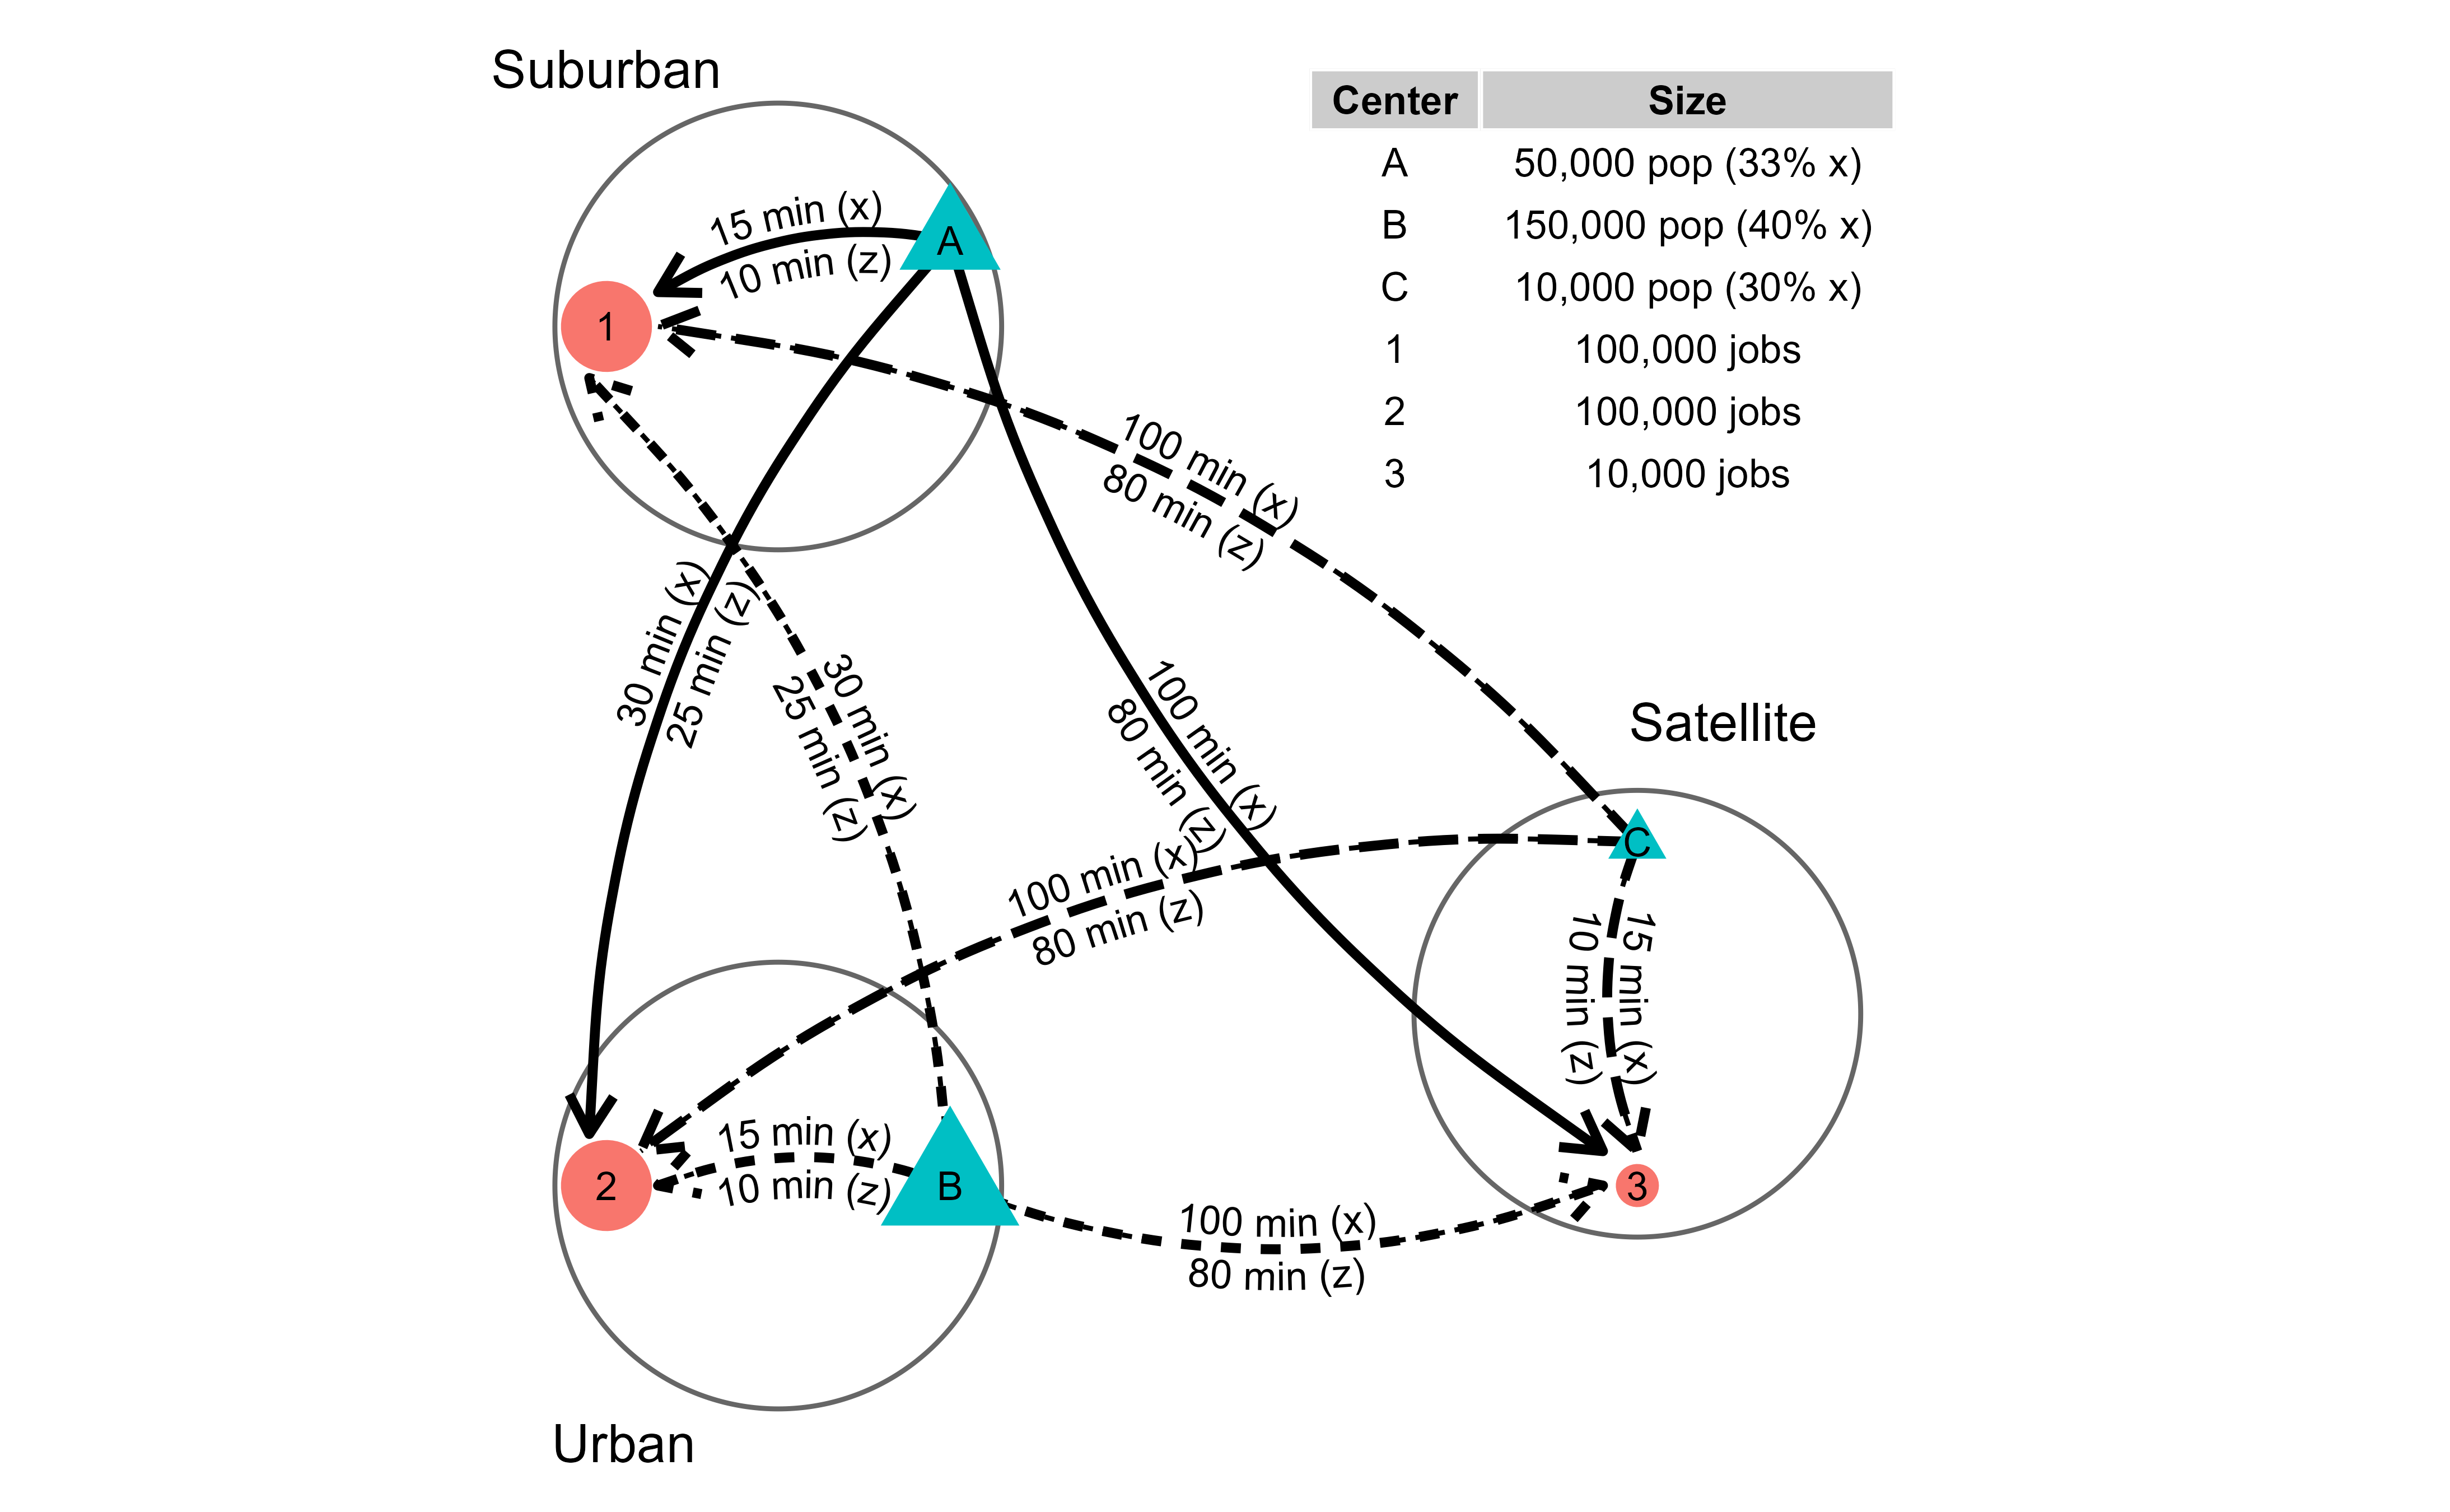
\includegraphics[width=1\linewidth]{images/Fig1} 

}

\caption{\label{fig:Fig1} Multimodal synthetic example: locations of employment centers (in orange), population centers (in blue), number of jobs and population, and travel times for two modes (slower mode x and faster mode z).}\label{fig:synthetic-example-plot}
\end{figure}

From the perspective of access to a \emph{finite} amount of
opportunities in the region (\(210,000\) jobs), the sub-population that
is most proximate to jobs, furthest from densely populated centers, and
is using the lowest travel-cost mode \(z\) can potentially access the
most job opportunities. This appears to be the sub-population at \(A\)
using mode \(z\). Sub-populations located in opposite conditions (i.e.,
further away from jobs, close to dense populations, and using \(x\)) are
at a relative job opportunity access \emph{disadvantage}. The
competition for opportunities between different mode-using populations
matters from the perspective of inequities as it reflects how well the
land-use and transport system serves (or doesn't serve) certain
populations.

\global\setlength{\Oldarrayrulewidth}{\arrayrulewidth}

\global\setlength{\Oldtabcolsep}{\tabcolsep}

\setlength{\tabcolsep}{0pt}

\renewcommand*{\arraystretch}{1.5}



\providecommand{\ascline}[3]{\noalign{\global\arrayrulewidth #1}\arrayrulecolor[HTML]{#2}\cline{#3}}

\begin{longtable}[c]{|p{0.88in}|p{0.41in}|p{1.05in}|p{0.58in}|p{1.05in}|p{0.58in}|p{1.05in}}

\caption{Accessibility\ values\ at\ each\ origin\ per\ mode\ m\ at\ each\ origin\ i\ and\ aggregated\ between\ modes\ for\ each\ i\ for\ the\ synthetic\ example.}\\

\ascline{1.5pt}{666666}{1-7}

\multicolumn{1}{>{\raggedright}m{\dimexpr 0.88in+0\tabcolsep}}{\textcolor[HTML]{000000}{\fontsize{11}{11}\selectfont{i}}} & \multicolumn{1}{>{\raggedright}m{\dimexpr 0.41in+0\tabcolsep}}{\textcolor[HTML]{000000}{\fontsize{11}{11}\selectfont{m}}} & \multicolumn{1}{!{\color[HTML]{666666}\vrule width 1pt}>{\raggedleft}m{\dimexpr 1.05in+0\tabcolsep}}{\textcolor[HTML]{000000}{\fontsize{11}{11}\selectfont{S}}\textcolor[HTML]{000000}{\textsubscript{\fontsize{11}{11}\selectfont{i}}}\textcolor[HTML]{000000}{\textsuperscript{\fontsize{11}{11}\selectfont{m}}}} & \multicolumn{1}{>{\raggedleft}m{\dimexpr 0.58in+0\tabcolsep}}{\textcolor[HTML]{000000}{\fontsize{11}{11}\selectfont{a}}\textcolor[HTML]{000000}{\textsubscript{\fontsize{11}{11}\selectfont{i}}}\textcolor[HTML]{000000}{\textsuperscript{\fontsize{11}{11}\selectfont{m}}}} & \multicolumn{1}{>{\raggedleft}m{\dimexpr 1.05in+0\tabcolsep}}{\textcolor[HTML]{000000}{\fontsize{11}{11}\selectfont{V}}\textcolor[HTML]{000000}{\textsubscript{\fontsize{11}{11}\selectfont{i}}}\textcolor[HTML]{000000}{\textsuperscript{\fontsize{11}{11}\selectfont{m}}}} & \multicolumn{1}{!{\color[HTML]{666666}\vrule width 1pt}>{\raggedleft}m{\dimexpr 0.58in+0\tabcolsep}}{\textcolor[HTML]{000000}{\fontsize{11}{11}\selectfont{a}}\textcolor[HTML]{000000}{\textsubscript{\fontsize{11}{11}\selectfont{i}}}} & \multicolumn{1}{>{\raggedleft}m{\dimexpr 1.05in+0\tabcolsep}}{\textcolor[HTML]{000000}{\fontsize{11}{11}\selectfont{V}}\textcolor[HTML]{000000}{\textsubscript{\fontsize{11}{11}\selectfont{i}}}} \\

\ascline{1.5pt}{666666}{1-7}\endfirsthead \caption[]{Accessibility\ values\ at\ each\ origin\ per\ mode\ m\ at\ each\ origin\ i\ and\ aggregated\ between\ modes\ for\ each\ i\ for\ the\ synthetic\ example.}\\

\ascline{1.5pt}{666666}{1-7}

\multicolumn{1}{>{\raggedright}m{\dimexpr 0.88in+0\tabcolsep}}{\textcolor[HTML]{000000}{\fontsize{11}{11}\selectfont{i}}} & \multicolumn{1}{>{\raggedright}m{\dimexpr 0.41in+0\tabcolsep}}{\textcolor[HTML]{000000}{\fontsize{11}{11}\selectfont{m}}} & \multicolumn{1}{!{\color[HTML]{666666}\vrule width 1pt}>{\raggedleft}m{\dimexpr 1.05in+0\tabcolsep}}{\textcolor[HTML]{000000}{\fontsize{11}{11}\selectfont{S}}\textcolor[HTML]{000000}{\textsubscript{\fontsize{11}{11}\selectfont{i}}}\textcolor[HTML]{000000}{\textsuperscript{\fontsize{11}{11}\selectfont{m}}}} & \multicolumn{1}{>{\raggedleft}m{\dimexpr 0.58in+0\tabcolsep}}{\textcolor[HTML]{000000}{\fontsize{11}{11}\selectfont{a}}\textcolor[HTML]{000000}{\textsubscript{\fontsize{11}{11}\selectfont{i}}}\textcolor[HTML]{000000}{\textsuperscript{\fontsize{11}{11}\selectfont{m}}}} & \multicolumn{1}{>{\raggedleft}m{\dimexpr 1.05in+0\tabcolsep}}{\textcolor[HTML]{000000}{\fontsize{11}{11}\selectfont{V}}\textcolor[HTML]{000000}{\textsubscript{\fontsize{11}{11}\selectfont{i}}}\textcolor[HTML]{000000}{\textsuperscript{\fontsize{11}{11}\selectfont{m}}}} & \multicolumn{1}{!{\color[HTML]{666666}\vrule width 1pt}>{\raggedleft}m{\dimexpr 0.58in+0\tabcolsep}}{\textcolor[HTML]{000000}{\fontsize{11}{11}\selectfont{a}}\textcolor[HTML]{000000}{\textsubscript{\fontsize{11}{11}\selectfont{i}}}} & \multicolumn{1}{>{\raggedleft}m{\dimexpr 1.05in+0\tabcolsep}}{\textcolor[HTML]{000000}{\fontsize{11}{11}\selectfont{V}}\textcolor[HTML]{000000}{\textsubscript{\fontsize{11}{11}\selectfont{i}}}} \\

\ascline{1.5pt}{666666}{1-7}\endhead



\multicolumn{1}{>{\raggedright}m{\dimexpr 0.88in+0\tabcolsep}}{} & \multicolumn{1}{>{\raggedright}m{\dimexpr 0.41in+0\tabcolsep}}{\textcolor[HTML]{000000}{\fontsize{11}{11}\selectfont{x}}} & \multicolumn{1}{!{\color[HTML]{666666}\vrule width 1pt}>{\raggedleft}m{\dimexpr 1.05in+0\tabcolsep}}{\textcolor[HTML]{000000}{\fontsize{11}{11}\selectfont{27,292.18}}} & \multicolumn{1}{>{\raggedleft}m{\dimexpr 0.58in+0\tabcolsep}}{\textcolor[HTML]{000000}{\fontsize{11}{11}\selectfont{0.95}}} & \multicolumn{1}{>{\raggedleft}m{\dimexpr 1.05in+0\tabcolsep}}{\textcolor[HTML]{000000}{\fontsize{11}{11}\selectfont{15,696.89}}} & \multicolumn{1}{!{\color[HTML]{666666}\vrule width 1pt}>{\raggedleft}m{\dimexpr 0.58in+0\tabcolsep}}{} & \multicolumn{1}{>{\raggedleft}m{\dimexpr 1.05in+0\tabcolsep}}{} \\





\multicolumn{1}{>{\raggedright}m{\dimexpr 0.88in+0\tabcolsep}}{\multirow[c]{-2}{*}{\parbox{0.88in}{\raggedright \textcolor[HTML]{000000}{\fontsize{11}{11}\selectfont{A}}}}} & \multicolumn{1}{>{\raggedright}m{\dimexpr 0.41in+0\tabcolsep}}{\textcolor[HTML]{000000}{\fontsize{11}{11}\selectfont{z}}} & \multicolumn{1}{!{\color[HTML]{666666}\vrule width 1pt}>{\raggedleft}m{\dimexpr 1.05in+0\tabcolsep}}{\textcolor[HTML]{000000}{\fontsize{11}{11}\selectfont{44,999.80}}} & \multicolumn{1}{>{\raggedleft}m{\dimexpr 0.58in+0\tabcolsep}}{\textcolor[HTML]{000000}{\fontsize{11}{11}\selectfont{1.57}}} & \multicolumn{1}{>{\raggedleft}m{\dimexpr 1.05in+0\tabcolsep}}{\textcolor[HTML]{000000}{\fontsize{11}{11}\selectfont{51,785.72}}} & \multicolumn{1}{!{\color[HTML]{666666}\vrule width 1pt}>{\raggedleft}m{\dimexpr 0.58in+0\tabcolsep}}{\multirow[c]{-2}{*}{\parbox{0.58in}{\raggedleft \textcolor[HTML]{000000}{\fontsize{11}{11}\selectfont{1.36}}}}} & \multicolumn{1}{>{\raggedleft}m{\dimexpr 1.05in+0\tabcolsep}}{\multirow[c]{-2}{*}{\parbox{1.05in}{\raggedleft \textcolor[HTML]{000000}{\fontsize{11}{11}\selectfont{67,482.61}}}}} \\

\ascline{1pt}{666666}{1-7}



\multicolumn{1}{>{\raggedright}m{\dimexpr 0.88in+0\tabcolsep}}{} & \multicolumn{1}{>{\raggedright}m{\dimexpr 0.41in+0\tabcolsep}}{\textcolor[HTML]{000000}{\fontsize{11}{11}\selectfont{x}}} & \multicolumn{1}{!{\color[HTML]{666666}\vrule width 1pt}>{\raggedleft}m{\dimexpr 1.05in+0\tabcolsep}}{\textcolor[HTML]{000000}{\fontsize{11}{11}\selectfont{27,292.18}}} & \multicolumn{1}{>{\raggedleft}m{\dimexpr 0.58in+0\tabcolsep}}{\textcolor[HTML]{000000}{\fontsize{11}{11}\selectfont{0.64}}} & \multicolumn{1}{>{\raggedleft}m{\dimexpr 1.05in+0\tabcolsep}}{\textcolor[HTML]{000000}{\fontsize{11}{11}\selectfont{38,170.03}}} & \multicolumn{1}{!{\color[HTML]{666666}\vrule width 1pt}>{\raggedleft}m{\dimexpr 0.58in+0\tabcolsep}}{} & \multicolumn{1}{>{\raggedleft}m{\dimexpr 1.05in+0\tabcolsep}}{} \\





\multicolumn{1}{>{\raggedright}m{\dimexpr 0.88in+0\tabcolsep}}{\multirow[c]{-2}{*}{\parbox{0.88in}{\raggedright \textcolor[HTML]{000000}{\fontsize{11}{11}\selectfont{B}}}}} & \multicolumn{1}{>{\raggedright}m{\dimexpr 0.41in+0\tabcolsep}}{\textcolor[HTML]{000000}{\fontsize{11}{11}\selectfont{z}}} & \multicolumn{1}{!{\color[HTML]{666666}\vrule width 1pt}>{\raggedleft}m{\dimexpr 1.05in+0\tabcolsep}}{\textcolor[HTML]{000000}{\fontsize{11}{11}\selectfont{44,999.80}}} & \multicolumn{1}{>{\raggedleft}m{\dimexpr 0.58in+0\tabcolsep}}{\textcolor[HTML]{000000}{\fontsize{11}{11}\selectfont{1.05}}} & \multicolumn{1}{>{\raggedleft}m{\dimexpr 1.05in+0\tabcolsep}}{\textcolor[HTML]{000000}{\fontsize{11}{11}\selectfont{94,468.91}}} & \multicolumn{1}{!{\color[HTML]{666666}\vrule width 1pt}>{\raggedleft}m{\dimexpr 0.58in+0\tabcolsep}}{\multirow[c]{-2}{*}{\parbox{0.58in}{\raggedleft \textcolor[HTML]{000000}{\fontsize{11}{11}\selectfont{0.88}}}}} & \multicolumn{1}{>{\raggedleft}m{\dimexpr 1.05in+0\tabcolsep}}{\multirow[c]{-2}{*}{\parbox{1.05in}{\raggedleft \textcolor[HTML]{000000}{\fontsize{11}{11}\selectfont{132,638.94}}}}} \\

\ascline{1pt}{666666}{1-7}



\multicolumn{1}{>{\raggedright}m{\dimexpr 0.88in+0\tabcolsep}}{} & \multicolumn{1}{>{\raggedright}m{\dimexpr 0.41in+0\tabcolsep}}{\textcolor[HTML]{000000}{\fontsize{11}{11}\selectfont{x}}} & \multicolumn{1}{!{\color[HTML]{666666}\vrule width 1pt}>{\raggedleft}m{\dimexpr 1.05in+0\tabcolsep}}{\textcolor[HTML]{000000}{\fontsize{11}{11}\selectfont{2,240.38}}} & \multicolumn{1}{>{\raggedleft}m{\dimexpr 0.58in+0\tabcolsep}}{\textcolor[HTML]{000000}{\fontsize{11}{11}\selectfont{0.68}}} & \multicolumn{1}{>{\raggedleft}m{\dimexpr 1.05in+0\tabcolsep}}{\textcolor[HTML]{000000}{\fontsize{11}{11}\selectfont{2,035.86}}} & \multicolumn{1}{!{\color[HTML]{666666}\vrule width 1pt}>{\raggedleft}m{\dimexpr 0.58in+0\tabcolsep}}{} & \multicolumn{1}{>{\raggedleft}m{\dimexpr 1.05in+0\tabcolsep}}{} \\





\multicolumn{1}{>{\raggedright}m{\dimexpr 0.88in+0\tabcolsep}}{\multirow[c]{-2}{*}{\parbox{0.88in}{\raggedright \textcolor[HTML]{000000}{\fontsize{11}{11}\selectfont{C}}}}} & \multicolumn{1}{>{\raggedright}m{\dimexpr 0.41in+0\tabcolsep}}{\textcolor[HTML]{000000}{\fontsize{11}{11}\selectfont{z}}} & \multicolumn{1}{!{\color[HTML]{666666}\vrule width 1pt}>{\raggedleft}m{\dimexpr 1.05in+0\tabcolsep}}{\textcolor[HTML]{000000}{\fontsize{11}{11}\selectfont{3,745.89}}} & \multicolumn{1}{>{\raggedleft}m{\dimexpr 0.58in+0\tabcolsep}}{\textcolor[HTML]{000000}{\fontsize{11}{11}\selectfont{1.12}}} & \multicolumn{1}{>{\raggedleft}m{\dimexpr 1.05in+0\tabcolsep}}{\textcolor[HTML]{000000}{\fontsize{11}{11}\selectfont{7,842.59}}} & \multicolumn{1}{!{\color[HTML]{666666}\vrule width 1pt}>{\raggedleft}m{\dimexpr 0.58in+0\tabcolsep}}{\multirow[c]{-2}{*}{\parbox{0.58in}{\raggedleft \textcolor[HTML]{000000}{\fontsize{11}{11}\selectfont{0.99}}}}} & \multicolumn{1}{>{\raggedleft}m{\dimexpr 1.05in+0\tabcolsep}}{\multirow[c]{-2}{*}{\parbox{1.05in}{\raggedleft \textcolor[HTML]{000000}{\fontsize{11}{11}\selectfont{9,878.45}}}}} \\

\ascline{1pt}{666666}{1-7}



\multicolumn{1}{>{\raggedright}m{\dimexpr 0.88in+0\tabcolsep}}{\textcolor[HTML]{000000}{\fontsize{11}{11}\selectfont{TOTALS}}} & \multicolumn{1}{>{\raggedright}m{\dimexpr 0.41in+0\tabcolsep}}{\textcolor[HTML]{000000}{\fontsize{11}{11}\selectfont{}}} & \multicolumn{1}{!{\color[HTML]{666666}\vrule width 1pt}>{\raggedleft}m{\dimexpr 1.05in+0\tabcolsep}}{\textcolor[HTML]{000000}{\fontsize{11}{11}\selectfont{150,570.22}}} & \multicolumn{1}{>{\raggedleft}m{\dimexpr 0.58in+0\tabcolsep}}{\textcolor[HTML]{000000}{\fontsize{11}{11}\selectfont{N/A}}} & \multicolumn{1}{>{\raggedleft}m{\dimexpr 1.05in+0\tabcolsep}}{\textcolor[HTML]{000000}{\fontsize{11}{11}\selectfont{210,000.00}}} & \multicolumn{1}{!{\color[HTML]{666666}\vrule width 1pt}>{\raggedleft}m{\dimexpr 0.58in+0\tabcolsep}}{\textcolor[HTML]{000000}{\fontsize{11}{11}\selectfont{N/A}}} & \multicolumn{1}{>{\raggedleft}m{\dimexpr 1.05in+0\tabcolsep}}{\textcolor[HTML]{000000}{\fontsize{11}{11}\selectfont{210,000.00}}} \\

\ascline{1.5pt}{666666}{1-7}



\end{longtable}



\arrayrulecolor[HTML]{000000}

\global\setlength{\arrayrulewidth}{\Oldarrayrulewidth}

\global\setlength{\tabcolsep}{\Oldtabcolsep}

\renewcommand*{\arraystretch}{1}

The calculated \(S_i^m\), \(a_i^m\) and \(V_i^m\) accessibility values
for each \(i\) and \(m\) are shown in the middle three columns and are
aggregated for each \(i\) in the final two columns in Table 1 . We use a
negative exponential impedance function
\(f^m(c_{ij}^m) = \exp(-\beta\cdot c_{ij})\) with \(\beta=0.1\) for both
\(x\) and \(z\) modes for all accessibility measures calculations.

The Hansen-type measure \(S_i^m\) is presented for each origin and mode
in third column of Table 1 . For all \(i\), the \(z\)-using
sub-population has higher \(S_i^m\) values than the \(x\)-using
sub-populations. Additionally, \(S_i^m\) is equal for both mode-using
populations in \(A\) and \(B\). This is the case since \(S_i^m\) does
not consider \emph{competition}, it only relies on reflecting the count
of opportunities that may be interacted with as a product of
\(f^m(c_{ij}^m)\). Recall, populations in \(A\) and \(B\) have the same
travel impedance to employment centers \(1\), \(2\) and \(3\) (either
15, 30, or 100 minutes using \(x\) or 10, 25, or 80 minutes using
\(z\)). As such, these the calculated \(S_i^m\) values are the same for
both \(A\) and \(B\). Furthermore, the total sum of \(S_i^m\) in the
region is equal to 150,570.2. This value is difficult to interpret: it
represents the weighted sum of opportunities that may be interacted with
within the region based on travel impedance. It cannot be interpreted as
any sort of benchmark since the measure is \emph{non-constrained}. To
connect this example to literature, \(S_i^m\) is calculated in the work
of {[}20{]}; they compare differences in \(S_i^m\) values between modes
in a relative and comparative sense, but make no further interpretation
of the \(S_i^m\) values.

In the fourth and sixth column in Table 1 the Shen-type measure is
calculated: first for both origin and mode \(a_i^m\) as well as
aggregated by the weighted mean mode-population (
\(\sum_m \frac{P_i^m}{P_i}*a_i^m\) ) to represent a value for each
origin \(a_i\). Unlike \(S_i^m\), this measure considers
\emph{competition}. For instance, the \(x\)-using populations in \(A\)
and \(B\) centers do not have the same \(a_i^m\) values as the
\(z\)-using. In fact, \(A\) has the highest values \(a_i^m\) and \(a_i\)
values since this center has the smallest travel impedance to
opportunities (lower than at \(C\), \(A\) and \(B\) are equal) and has
one of these lowest proximity to a relatively high amount of population
(lower than at \(B\)).

However, the Shen-type measure is \emph{non-constrained}: the total sum
of \(a_i^m\) or \(a_i\) is practically meaningless since it represents a
sum of ratios. For instance, the \(z\)-using sub-population at \(A\) has
a value of 1.57 potential jobs per potential job-seeking population
compared to 0.95 for \(x\)-using sub-population. What is the
significance of these values? The difference between these modes is
equal to 0.62, but 0.62 of what? How many more job opportunities are
\(z\) users interacting with than \(x\) users? When \(a_i^m\) is
aggregated to \(a_i\) as shown in the sixth column, the values face
similar interpretability issues. The Shen-type measure is implemented in
the previously discussed work of {[}30{]} to calculate modal \(a_i^m\)
values and the aggregated \(a_i\) is implemented in the work of
{[}31{]}. However, similar to the Hansen-type measure, these works
discuss relative and spatially comparative differences in values, they
do not make further interpretation of the \(a_i^m\) or \(a_i\)
themselves. This may be because the Shen-type measure is
\emph{non-constrained}, this is no benchmark or global maximum to which
comparisons can be drawn from.

By contrast, spatial availability \(V_i\) considers competition and is
constrained such that the total sum of values is equal to the total
number of opportunities in the region (i.e., \(210,000\) jobs). Seen in
fifth column of Table 1 , \(V_i^m\) for the same mode-using populations
in \(A\) and \(B\) are not the same (as this measure considers
competition). In fact, at \(A\), the \(z\)-using sub-population captures
36,088.84 more spatially available jobs (of the \(210,000\) jobs in the
region) than the sub-population using mode \(x\). The numerical
difference has a practical interpretation.

Furthermore, \(V_i^m\) values for an \(i\) can be aggregated across
\(m\) and compared across \(i\) ( \(V_i = \sum_m{\sum_i{V_i^m}}\) ) as a
result of the proportional allocation mechanism. This aggregation,
\(V_i\), is shown in the seventh column in Table 1 . Again looking at
center \(A\), \(A\) is allocated 67,482.61 spatially available
opportunities for both modes. 77\% of this spatial availability
allocated to \(A\) is assigned to the \(z\)-using population despite
representing 66\% of \(A\)'s population.

Spatial availability can be further aggregated to better interpret
competition between modes. Across the entire region, 130,000 people use
\(z\) (62\% of the region population). However, the \(z\)-using
population accounts for 73\% of the region's total spatial availability
- the rest is allocated to the \(x\)-using population (38\%of the total
population). Notably, the \(x\)-using population captures 11\% less
spatial availability to opportunities than its population proportion.
This understanding can lead us to ask normative questions such as, how
unequal should opportunity access for the two mode-using populations be?
Can the lower-travel-cost populations spare some spatial availability if
a policy of modal-restriction (like a LEZ) was introduced?

Since spatial availability is constrained and has an interpretable
meaning as a proportion of the total opportunities in the region, the
values at \(i\) have a new significance. Inequality in \(V_i^m\) values
can be explored through a variety of approaches. For instance, consider
travel times. The \(z\)-using population accounts for 67\% of the
potential travel time traveled in the region: this is 7\% less travel
time than the proportion of spatial available opportunities that is
allocated to them. In other words, the \(z\)-using population travels
less minutes overall and has more spatial availability of opportunities
than the \(x\)-using population using the slower mode \(x\).

Alternatively, inequities in spatial availability between mode-using
populations can be explored through proportional benchmarks. A spatial
availability per capita \(v_i^m\) as presented in Equation
(\ref{eq:SA-per-capita}):

\begin{equation}
\label{eq:SA-per-capita}
v_{i}^m = \frac{V_{i}^m}{P_{i}^m}
\end{equation}

The \(v_i^m\) values for \(A\), \(B\), and \(C\) for the \(x\)-using
sub-populations are 0.95, 0.64 and 0.68 spatially available jobs per
capita, respectively. The \(v_i^m\) for the \(z\)-using sub-populations
are much higher, with values of: 1.57, 1.05 and 1.12 respectively. The
\(x\)-using population, especially at \(B\) and \(C\), are directly
impacted by the jobs that are spatially available to the \(z\)-using
population \emph{in addition to} the mass effect (occurring at \(B\),
high population density) and high travel impedance (occurring at the
Satellite \(C\)).

If, lets say, the planning goal is to have one spatially available job
per mode-using population, a policy intervention can be put in place, to
reduce the \(v_i^z\) values and increase \(v_i^x\) values. This
demonstration is to show how simply the \(V_i^m\) framework can be
manipulated quantify the competitive (dis)advantage in a multimodal
application. In what follows, we further explore competition between
multiple modes through an empirical example.

\hypertarget{empirical-example-madrid-lez}{%
\section{Empirical example: Madrid
LEZ}\label{empirical-example-madrid-lez}}

\hypertarget{multimodal-data-and-methods}{%
\subsection{Multimodal data and
methods}\label{multimodal-data-and-methods}}

Low emission zones (LEZ) have been implemented as a climate change
policy intervention to reduce GHG emissions, improve air quality, and
support sustainable mobility in many countries {[}32,33{]}. Though rules
of exclusion vary, LEZ aim to deter/reduce traffic in designated zones
under threat of penalty (e.g., fines, seizure of vehicle). From the
perspective of restriction for passenger transport, LEZ are a policy of
\emph{geographic discrimination} as they change how people access
opportunities by making the travel impedance more costly for specific
car-mode users. When considering opportunities as finite in a region,
this discrimination could allow certain populations to access
opportunities by other modes more readily than before. In this way, LEZ
change the multimodal competitive accessibility landscape of a city.

Spain is one of a few countries with active LEZ and plans to expand
their implementation as specified in their climate-change-related plans:
\emph{Plan Nacional Integrado de Energía y Clima 2021-2030} {[}34{]} and
\emph{Plan Nacional de Control de la Contaminación Atmosférica}
{[}35{]}. Specifically, the national Spanish law 7/2021 ( \emph{Ley de
Cambio Climático y Transición Energética}) will require all
municipalities to implement LEZ by 2023 if they meet at least one of the
following requirements: (i) municipalities \textgreater50,000 inhab.;
(ii) islands; and (iii) municipalities \textgreater{} 20,000 inhab. when
air quality exceeds limits specified in \emph{RD 102/2011 de Mejora de
Calidad del Aire} {[}36{]}.

In 2017, LEZs were implemented in the Spanish capital city of Madrid
following the goals set out in the national agenda . In geographic
scope, the 2017 boundaries of the LEZ were relatively small (covering
4.72 km\(^2\)) and within the center (i.e., LEZ Centro). These
boundaries were expanded in 2023 to inside of the M-30, a highway in
proximity to the city center (i.e., LEZ M-30) and the city has plans to
further spatially expand the LEZ. Within the 2017 LEZ Centro
implementation, all cars, motorcycles and freight with environmental
label A or B (higher polluting classification, associated with older
make and model of fossil fuel internal combustion engine vehicles), are
not permitted to enter the area unless they are used by residents or
meet other exemptions. This restriction impacted approximately half of
all car trips that were typically made into the LEZ Centro {[}37{]}.

For this case study, we use \(V_i^m\) to quantify the competition of
spatially available opportunities between modes after the LEZ Centro
implementation. Particularly, we demonstrate how \(V_i^m\) can be used
to spectate on how the restriction of car mobility in areas
around/within the LEZ Centro allowed the other, more sustainable but
often with higher travel impedance modes, to become more competitive.

\begin{figure}

{\centering 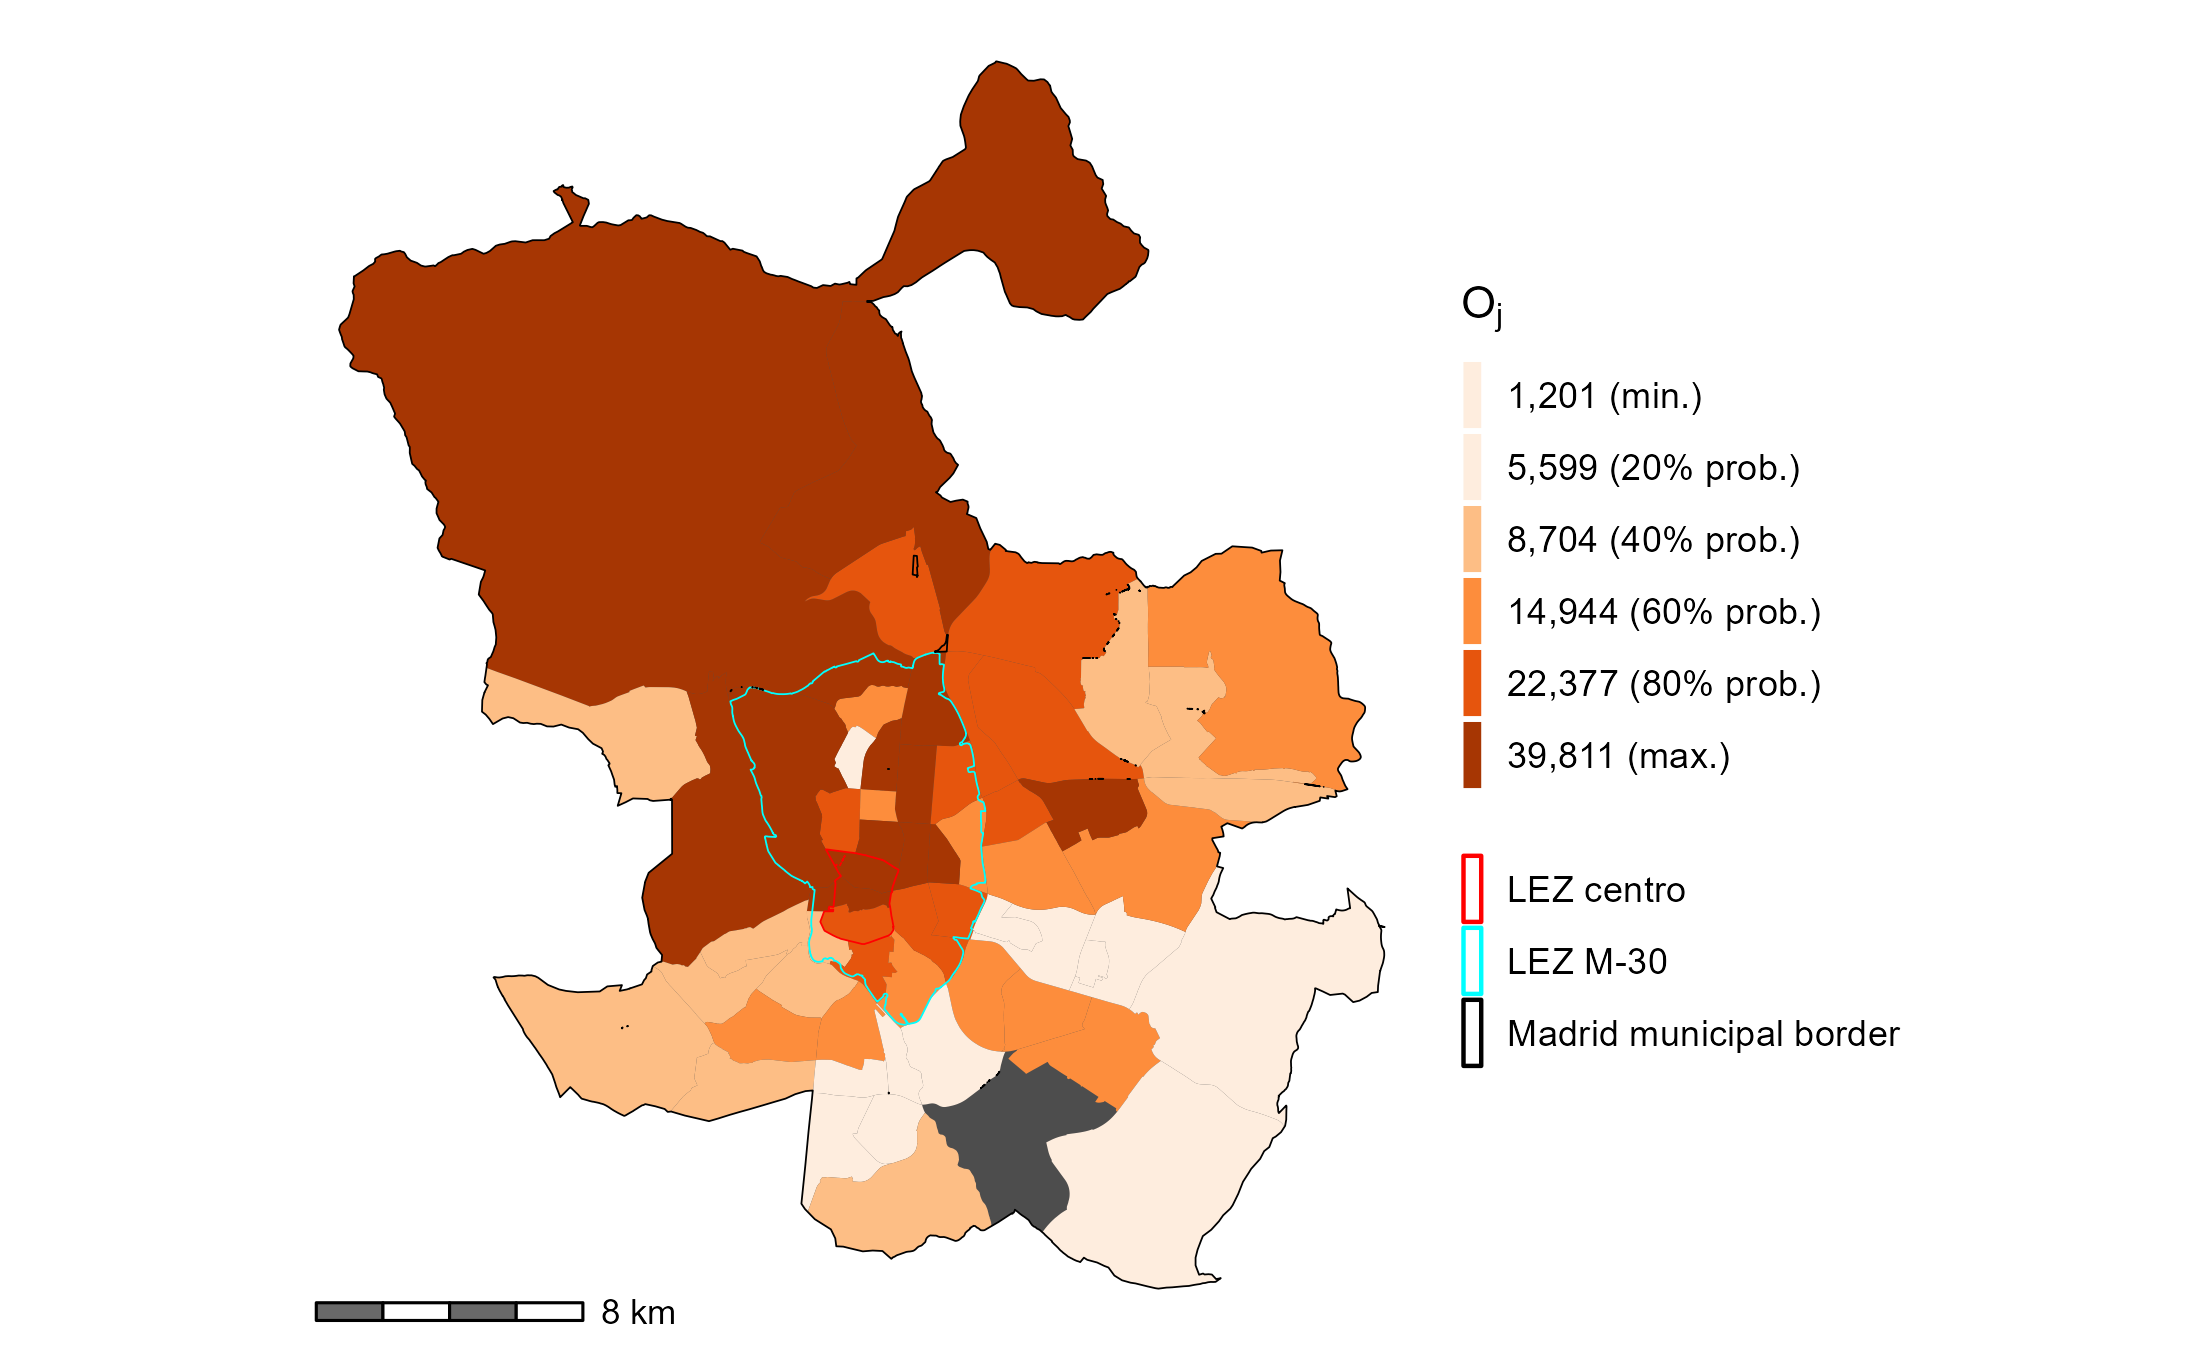
\includegraphics[width=1\linewidth]{images/i_jobs_zn208_plot} 

}

\caption{\label{fig:Fig2} Jobs $O_j$ taken by people living and working in Madrid as reported by the home-to-work flows in the 2018 travel survey. Gray TAZ has no jobs.}\label{fig:jobs-plot}
\end{figure}

\begin{figure}

{\centering 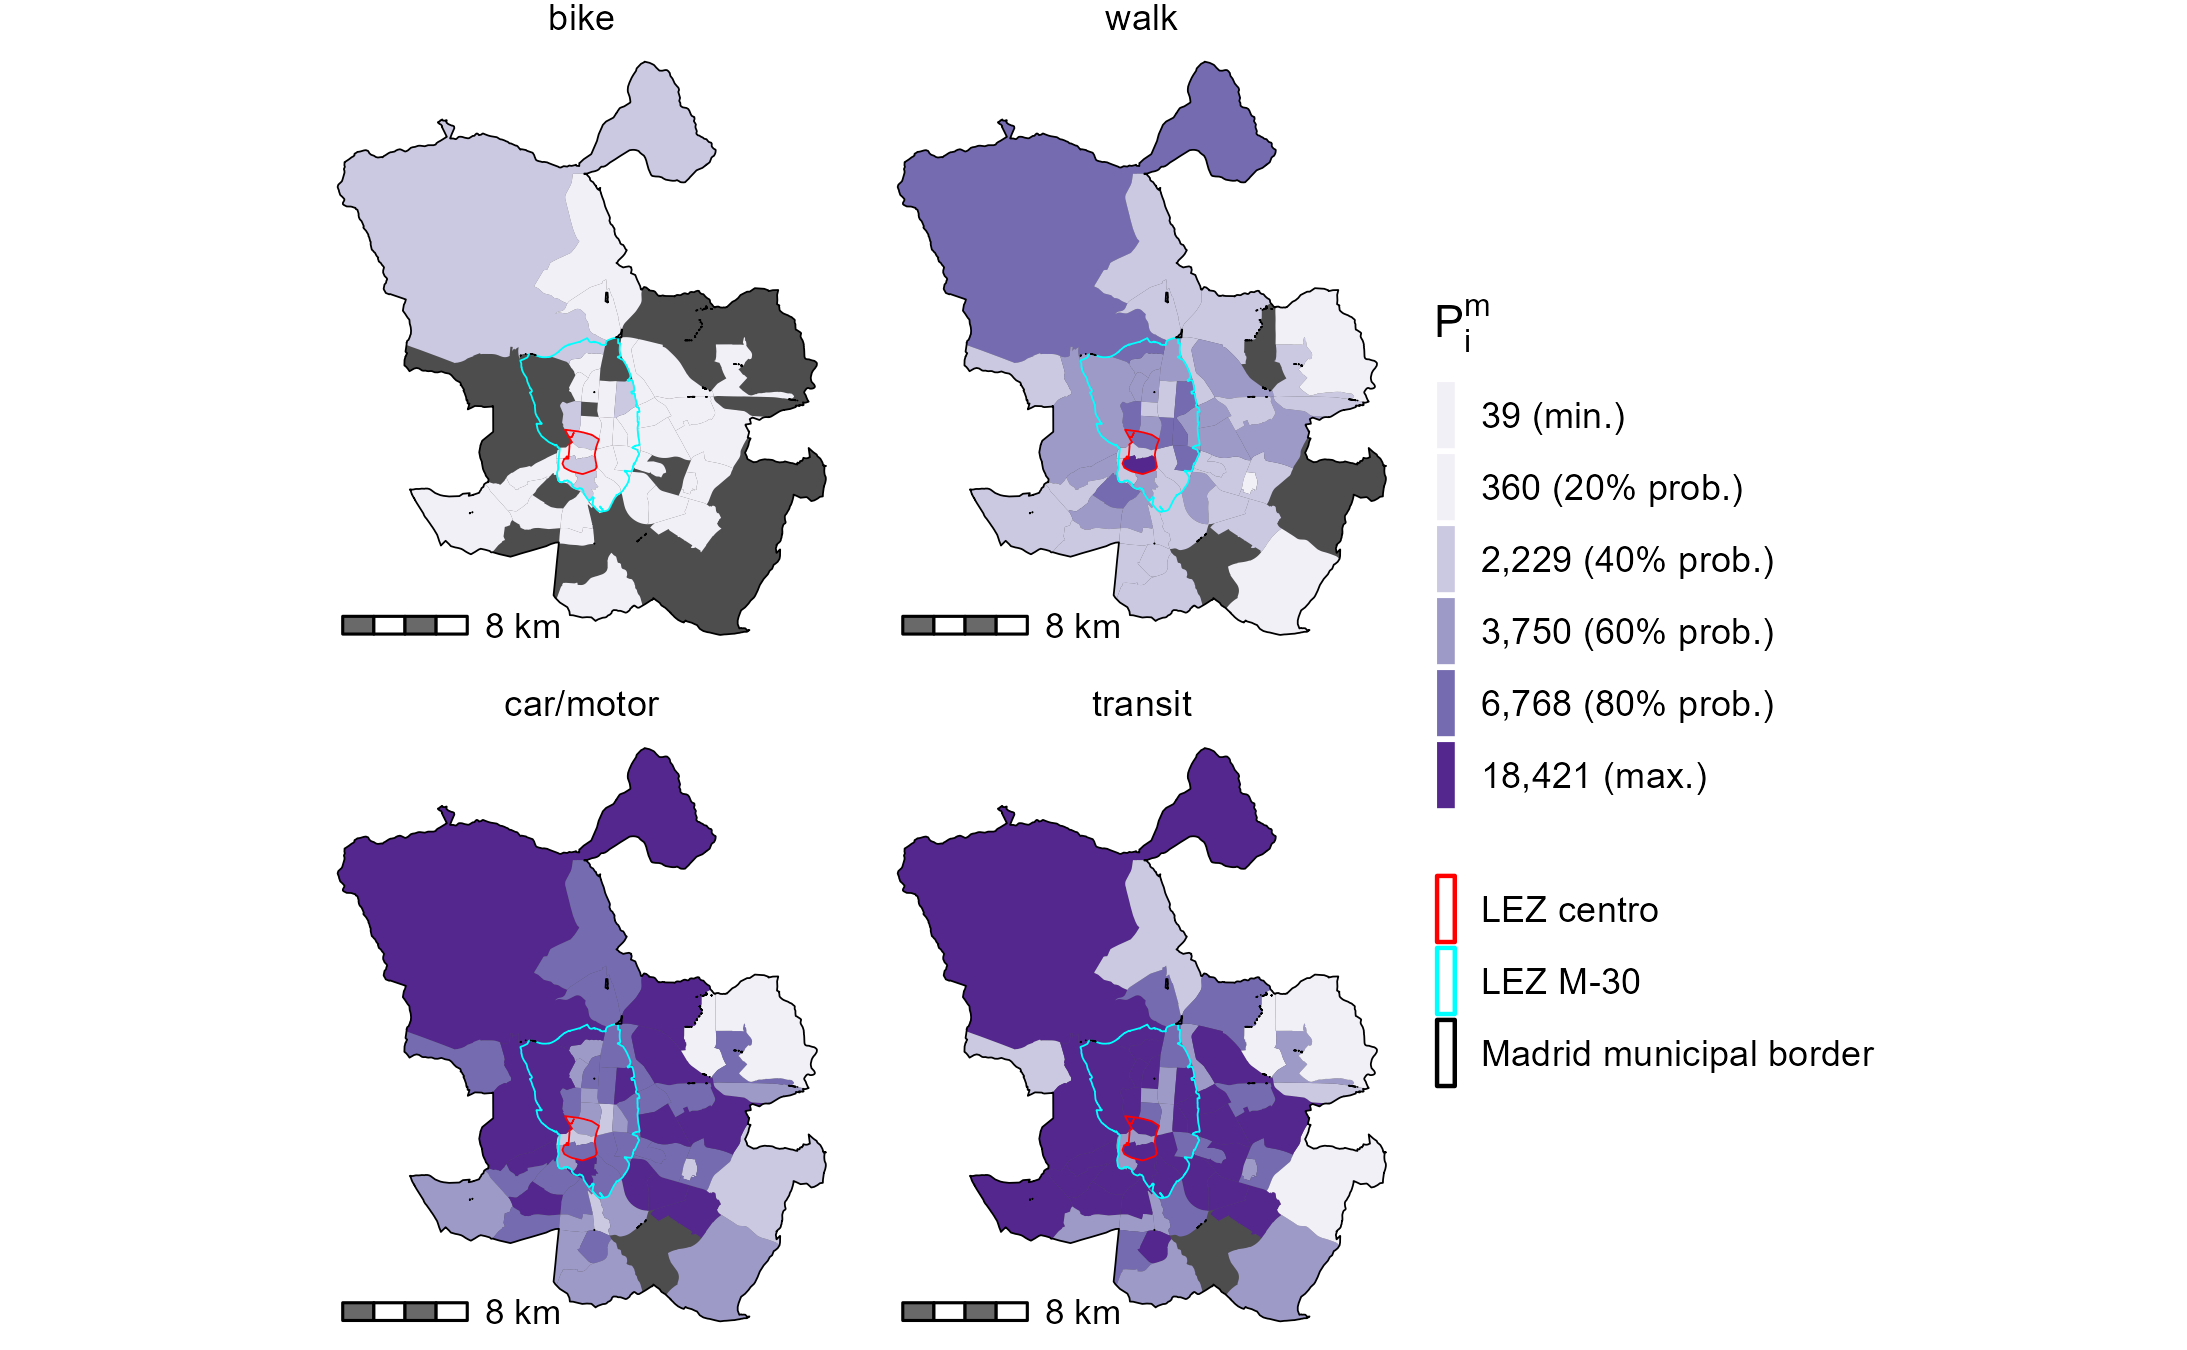
\includegraphics[width=1\linewidth]{images/im_populations_zn208_plot} 

}

\caption{\label{fig:Fig3} Population living and working in Madrid by four summarized modal categories $P^m_i$ as reported by the home-to-work flows in the 2018 travel survey. Gray TAZs have no population.}\label{fig:pop-plot}
\end{figure}

The 2018 Community of Madrid travel survey {[}38{]} is the source of
data for this empirical example: it is a representative survey that
reflects a snap-shot of the travel patterns for a typical day of the
working week in 2018. Specifically, it includes 222,744 trips taken from
a representative sample of 85,064 households across the traffic analysis
zones (TAZ) representing the Community of Madrid (population of
6,507,184 over 3 years old) through population elevation factors.

In this empirical example, we only use a sub-set of the survey,
specifically home-to-full-time-work trips, by all modes, to demonstrate
multimodal spatial availability of employment opportunities. The total
population who travels to full-time work from an origin (i.e., the
worker), and the destinations (i.e., the employment opportunity), for
the City of Madrid (a sub-set of the Community of Madrid) is visualized
in Figure \ref{fig:Fig2} and Figure \ref{fig:Fig3}. Both figures are
displayed at the level of TAZ (the \(i\) and \(j\) zones) that
correspond to the survey. The red boundary represents the LEZ Centro in
effect in 2017 and thus those travel patterns of car-restriction
reflected in the survey. The cyan boundary represents the LEZ that will
be within the boundaries of the M-30 highway in 2023 and is present in
the plots as a spatial reference for areas in proximity to the LEZ
Centro.

The total sum of jobs \(O_j\) that are held are shown in Figure
\ref{fig:Fig2} and the populations that go to a work destination by four
modal categories \(P^m_i\), is reflected in Figure \ref{fig:Fig3}. The
four modal categories represented in Figure \ref{fig:Fig3} are created
through the grouping of similar mode types as provided in the survey, by
the authors discretion. The modal categories and the mode types within
each category are reported as follows:

\begin{itemize}
\tightlist
\item
  Car/motor: all cars and operating modes (e.g., cab, private driver,
  company, rental car, main driver of a private car, passenger in a
  private car) and all public, private or company motorcycle/mopeds.
\item
  Transit: all bus, trams, and trains,
\item
  Bike: all bicycle trips (e.g., private, public, or company bike trips)
  and ``other'' types of micromobility options,
\item
  Walk: walking or by foot.
\end{itemize}

From Figure \ref{fig:Fig2}, it can be seen that the largest
concentration of jobs are within, near, and to the north of the LEZ
Centro. The population that is accessing those jobs by mode (Figure
\ref{fig:Fig3}), appear spatially distinct. Car and transit trips
represent 37\% and 47\% of the modal share respectively. The population
that travels using transit is more spatially distributed than those
using cars - particularly near and within LEZ Centro. This distribution
is likely caused by a variety of factors including: transit coverage and
service within with city, effective car infrastructure outside of the
M-30, and/or the impact of the LEZ Centro itself. From Figure
\ref{fig:Fig3}, it can be observed that biking and walking trips are
less common than motorized trips at 1\% and 15\% respectively. Noteably,
there is a positive trend between the populations of walking and biking
trips in zones and populations of transit trips. This positive trend is
higher than for car trip populations.

The travel time for each trip is provided within the survey. These
travel times, per modal category, are used to calibrate mode-specific
travel impedance functions \(f^m(c_{ij}^m)\). To illustrate the modal
differences in travel time lengths, summary descriptive per mode are
detailed:

\begin{itemize}
\tightlist
\item
  Car/motor: mean 36 minutes (min:0 minutes, Q2: 15 minutes, Q3: 55
  minutes, max: 120 minutes)
\item
  Transit: mean 55 minutes (min:1 minutes, Q2: 30 minutes, Q3: 80
  minutes, max: 120 minutes)
\item
  Bike: mean 34 minutes (min:5 minutes, Q2: 15 minutes, Q3: 40 minutes,
  max: 115 minutes)
\item
  Walk: mean 27 minutes (min:1 minutes, Q2: 10 minutes, Q3: 45 minutes,
  max: 119 minutes)
\end{itemize}

To calculate \(f^m(c_{ij}^m)\) from the survey travel times, a concept
known as the trip length distribution (TLD) is used. A TLD represents
the proportion of trips that are taken at a specific travel cost such as
travel time (i.e., probability density distribution of trips taken by
travel cost). This distribution is then used in the derivation of travel
impedance functions (e.g., done in the accessibility works of {[}39{]},
{[}40{]}, and {[}41{]}). To fit the impedance functions, we use the
Maximum likelihood estimation and the Nelder-Mead method for direct
optimization available within the R \{fitdistrplus\} package {[}42{]}.
Based on goodness-of-fit criteria and associated diagnostics, the gamma
and log-normal probability density functions are selected as best
fitting curves for the motorized and non-motorized modes respectively.
The selection of functional form aligns with empirical examples in other
regions {[}14,43,44{]}. The shape and rate parameters for the gamma
functions (motorized modes) are 1.8651852 and 0.051468for car/motor and
2.7566235 and 0.0499193 for transit; for the log-normal functions
(non-motorized modes), mean and standard deviation parameters are
3.2372212 and 0.7575986 for bike and 2.9918042 and 0.7575986 for walk.

Represented in Figure \ref{fig:Fig4} are four plots visualizing the
estimated probability density functions (represented as black lines)
over top the binned travel time data from the 2018 survey. The estimated
probability density functions can be interpreted as the probability of
travel (y-axis) given a trip travel time (x-axis), based on trip flows
from the 2018 travel survey. These `probability of travel' at each
travel time for each mode are realized observations that reflect the
land-use, the transport system, and the population travel behaviour in
Madrid (according to the 2018 survey). A trip that leaves \(i\) is
assigned a probability of travel value (y-axis) based on the mode and
travel time of that trip to work: this probability value is the input
\(f^m(c_{ij}^m)\).

Notably, plots in Figure \ref{fig:Fig4} can be observed across modes if
curious to know what trips are more likely to occur using what mode
depending on trip length (as informed by the observed 2018 survey).
Trips \textgreater5 minutes do not occur frequently for any mode, as
such trips with short trip lengths are assigned a lower travel impedance
\(f^m(c_{ij}^m)\) value. One reason that \textgreater5 minute trips do
not frequently occur as a result of land-use (residential and job
mismatch): not everyone lives in immediate proximity to their workplace.
In terms of the non-motorized modes, shorter trips occurred more
frequently overall for walking populations, particularly around 15
minute lengths, so a trip of approximately 15 minutes is assigned the
highest \(f^m(c_{ij}^m)\). For biking populations, longer travel times
are more common so though the highest \(f^m(c_{ij}^m)\) value also
corresponds to approximately 15 minutes, the curve is more spread out
and values decrease less rapidly at longer travel times than for the
walk mode curve. A similar trend can be observed for the motorized modal
options where transit mode is more spread out than car/motor mode. All
in all, these observations demonstrate that, based on a given mode and
travel time, a trip is more or less likely to occur and is accordingly
represented in the cost of travel balancing factor \(F_{ij}^m\) for
\(V_i^m\).

\begin{figure}

{\centering 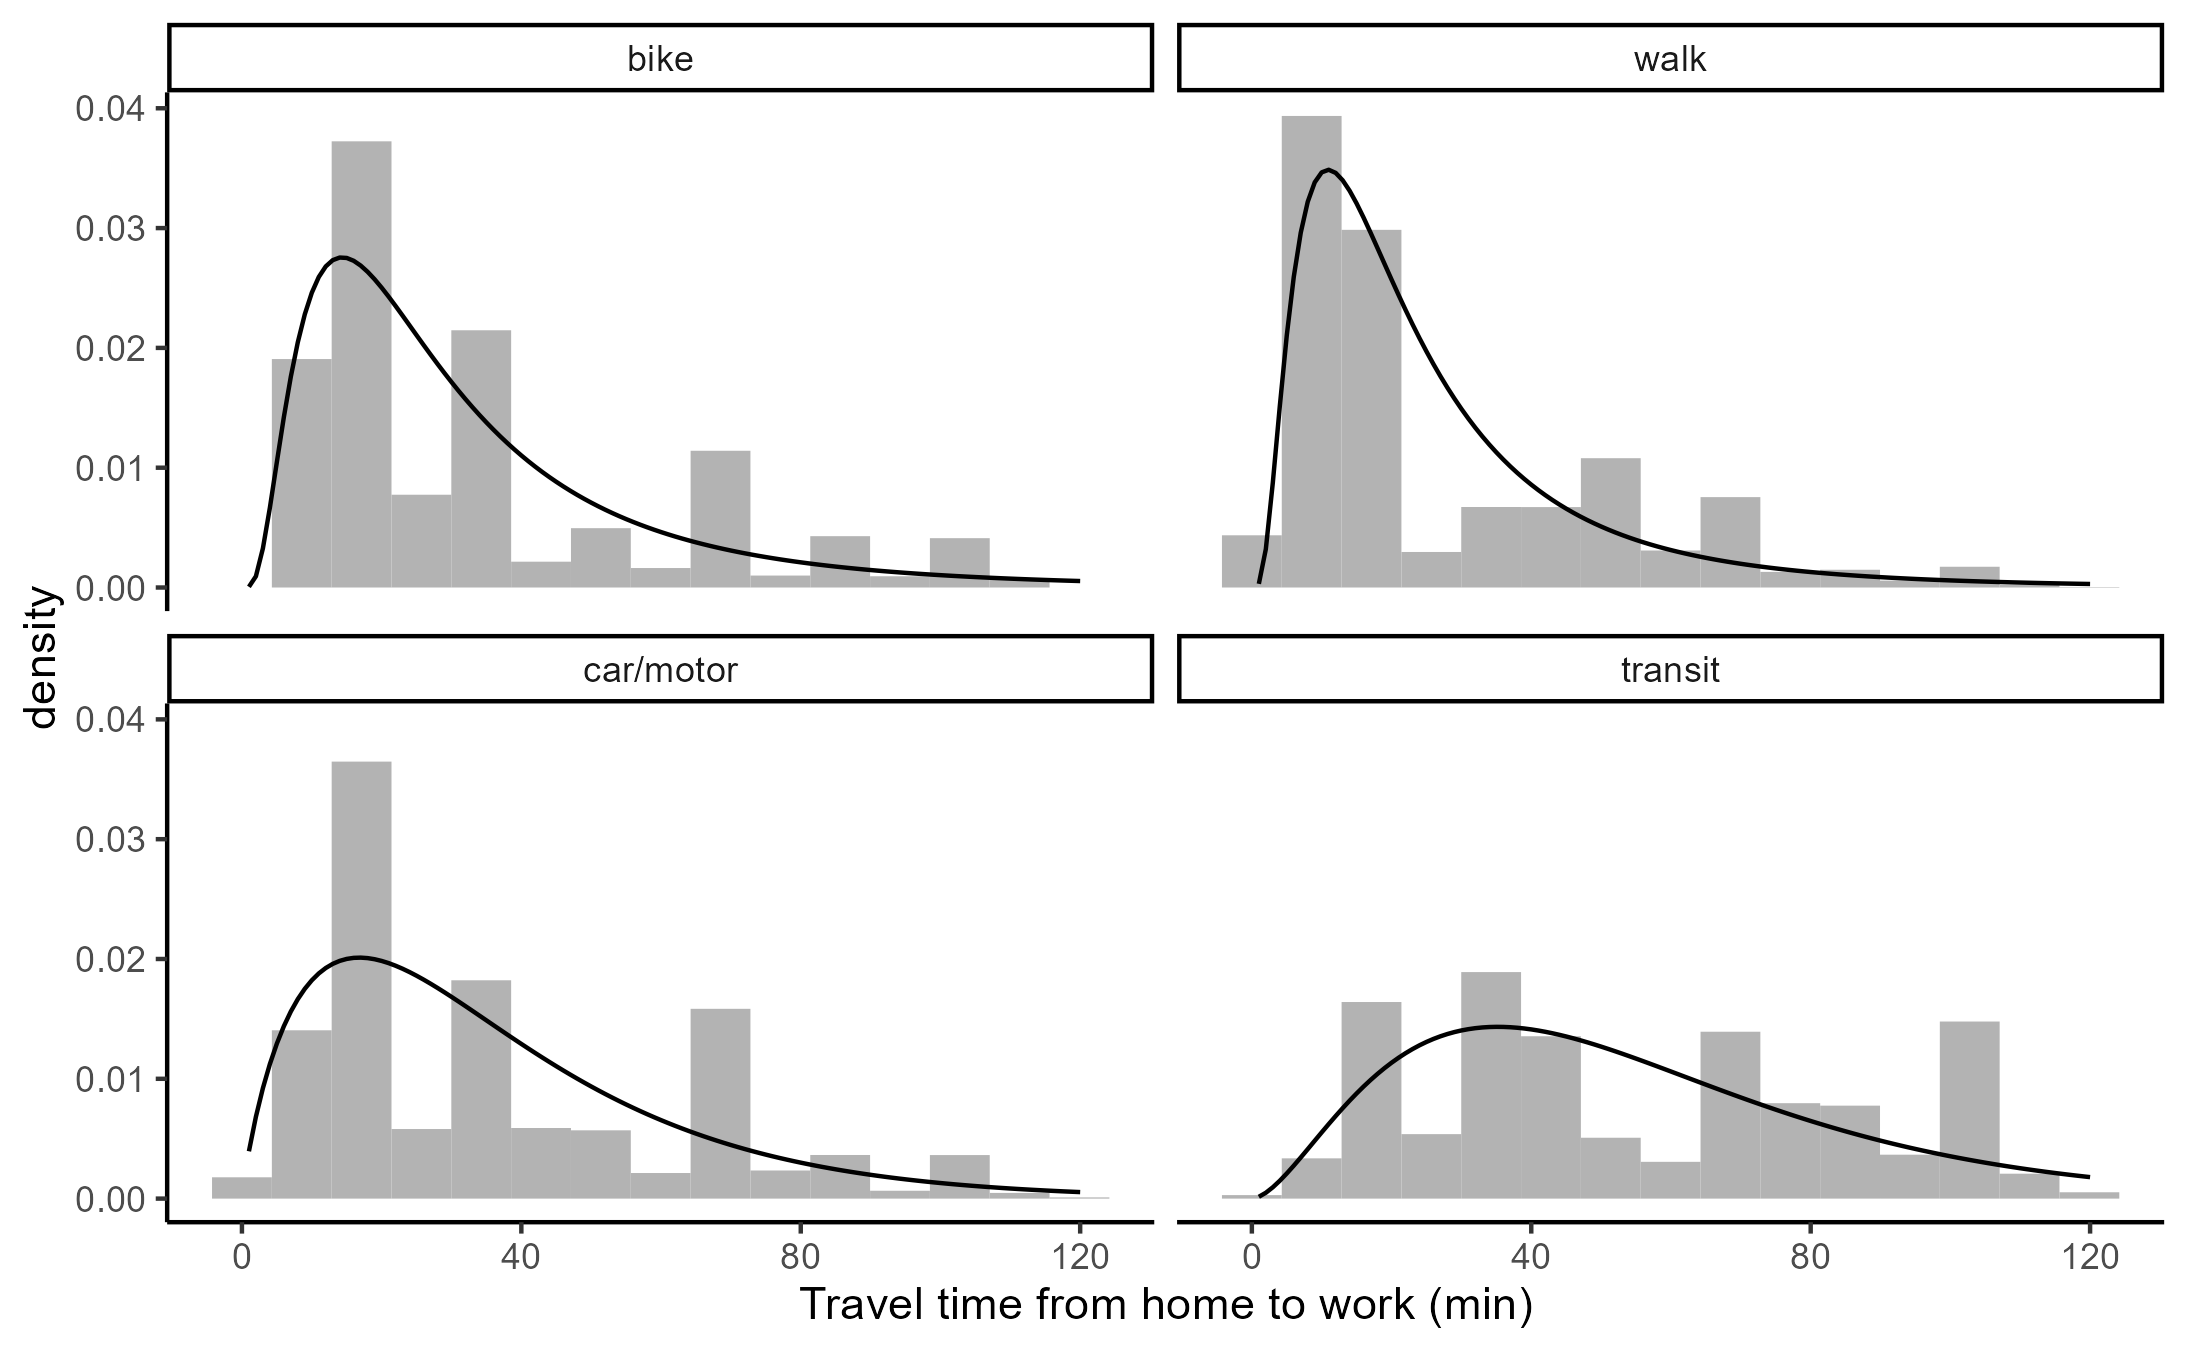
\includegraphics[width=1\linewidth]{images/tlds_curves_m_plot} 

}

\caption{\label{fig:Fig4} Fitted impedance function curve (line) against empirical TLD (bars) corresponding to the home-to-work origin-destination flows from the Madrid 2018 travel survey.}\label{fig:tlds-curves-m-plot}
\end{figure}

\hypertarget{results}{%
\subsection{Results}\label{results}}

As it is worth re-iterating, the empirical example reflects a snap-shot
of the calculated multimodal spatial availability using data from the
2018 travel survey. It is intended to visualize the spatial trends in
availability of employment opportunities, by mode, and demonstrate how
spatial availability can be interpreted to discuss the competitive
advantage of lower travel impedance modes within Madrid Centro.

The spatial availability of jobs \(V_i^m\) is calculated for each of the
four modal categories \(m\) at the level of traffic analysis zones \(i\)
in Madrid and demonstrated in Figure \ref{fig:Fig5}.

\begin{figure}

{\centering 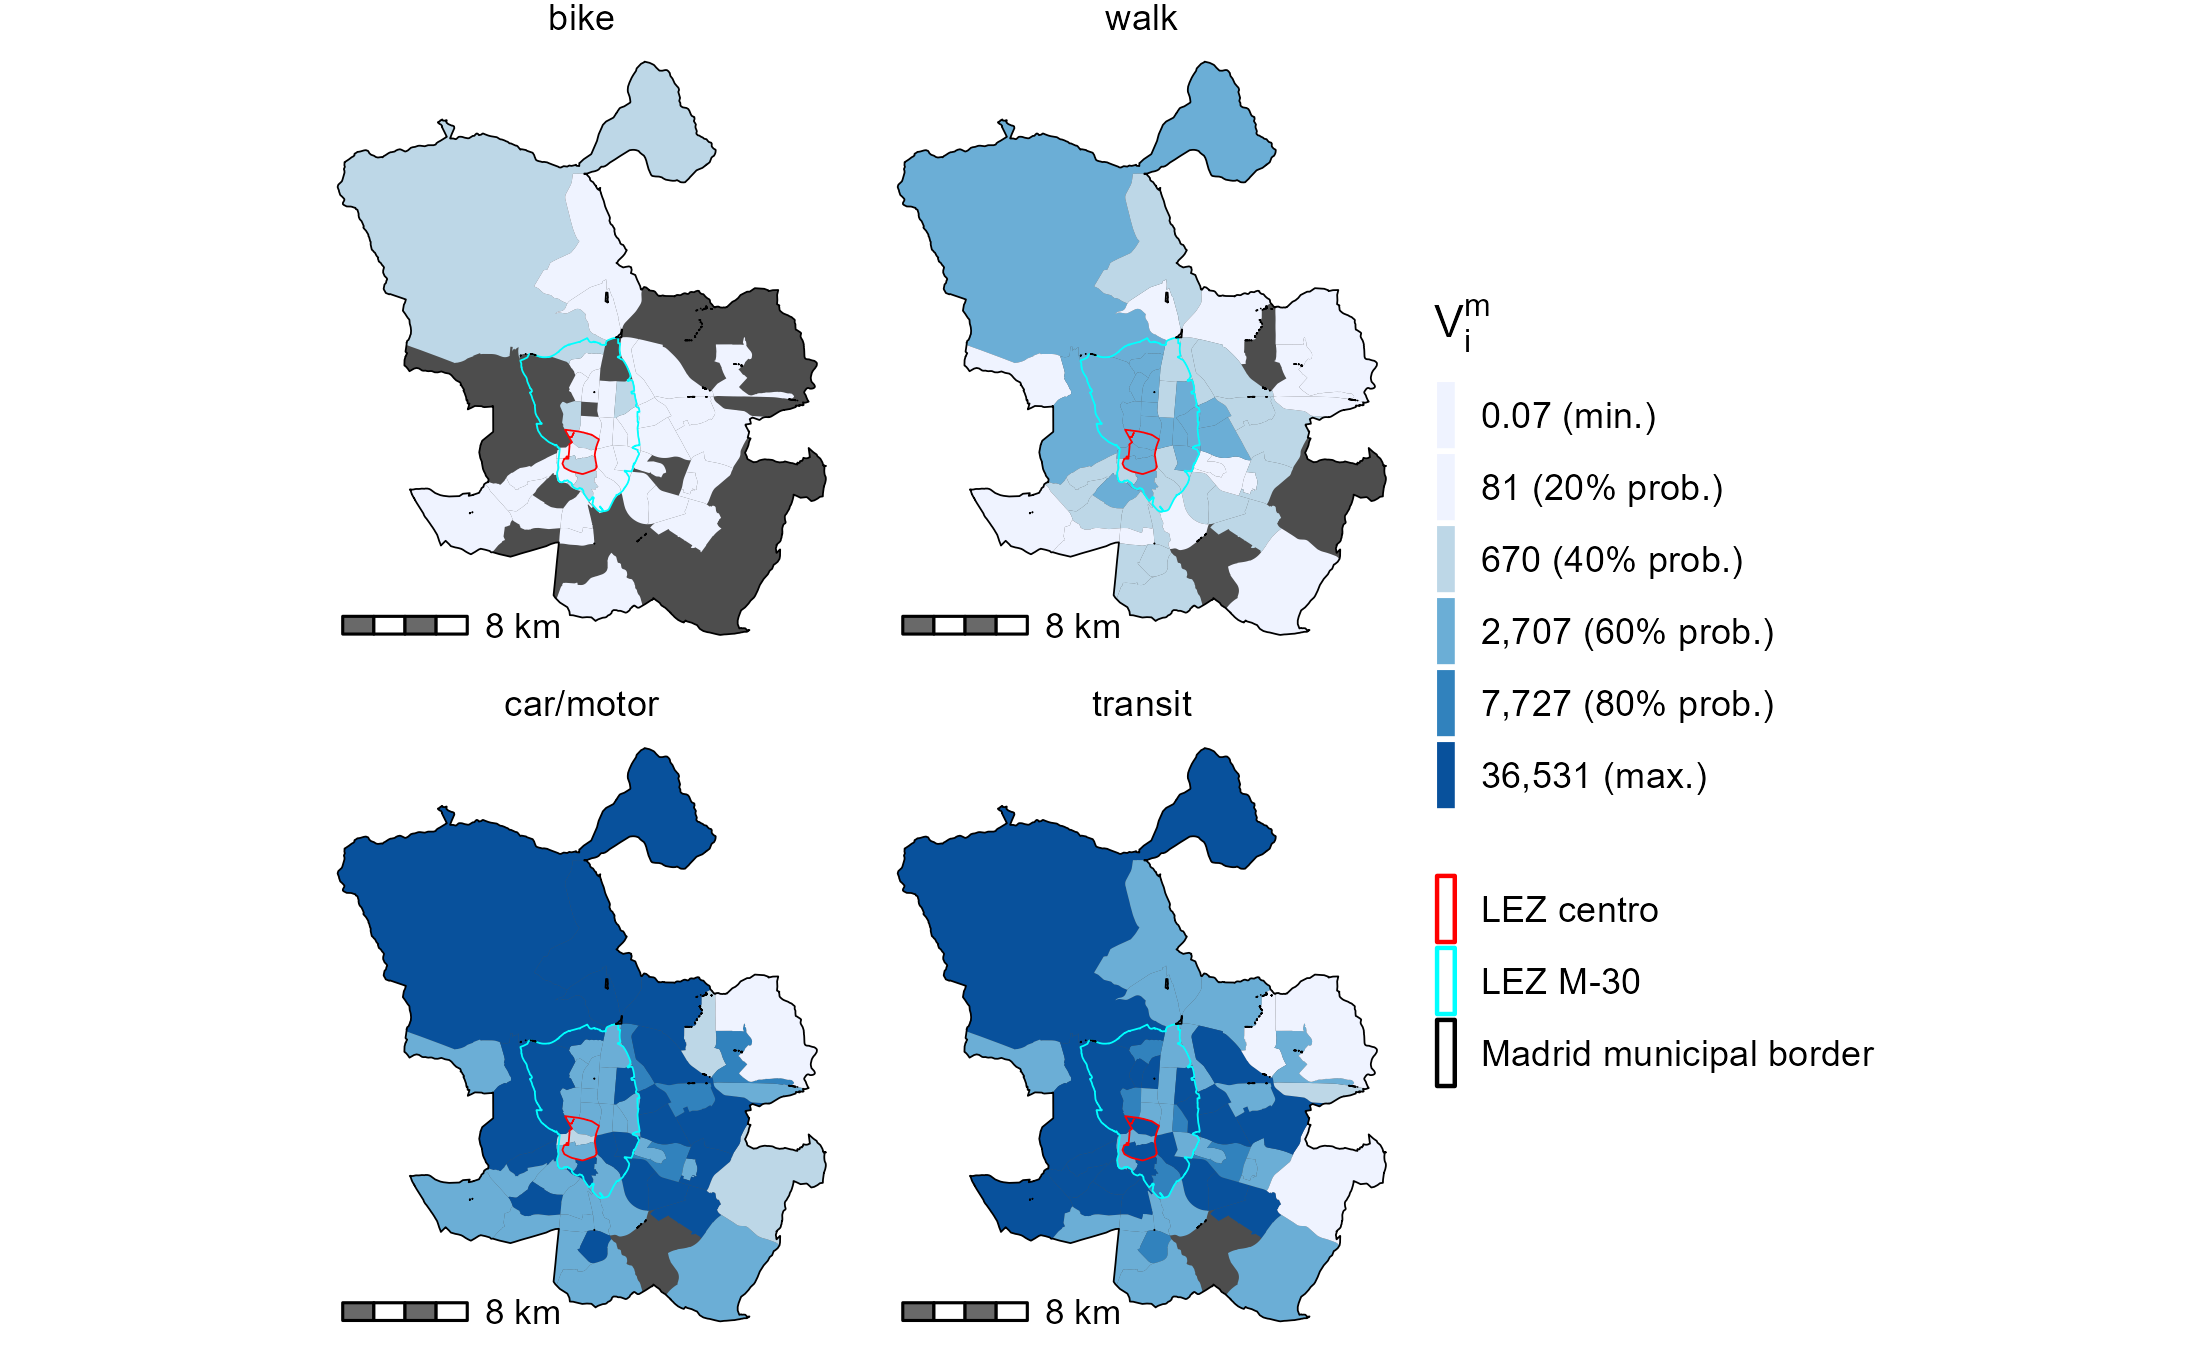
\includegraphics[width=1\linewidth]{images/SA_im_V_zn208_plot} 

}

\caption{\label{fig:Fig5} Spatial availability of job opportunities per origin and mode $V_i^m$ in Madrid. Calculated using the home-to-work flows from the 2018 travel survey. Gray TAZs have no population.}\label{fig:SA-m-plot}
\end{figure}

\(V_i^m\) is a proportion of the total number of 847,574 jobs in the
region and is visualized in Figure \ref{fig:Fig5}. Since \(V_i^m\) is
calculated based on the likelihood of travel from observed home-to-work
journeys, the values can be understood as the number of full-time jobs
that are spatially available to the full-time working population at that
\(i\) and their associated \(m\), relative to all the jobs in the city.
\(V_i^m\) is the number of jobs that are \emph{spatially available} to a
\(m\)-using population located at \(i\), relative to the travel
impedance and size of \emph{all} populations in the region.

Notable are the differences in the magnitude of \(V_i^m\) between modes
in Figure \ref{fig:Fig5}. The majority of \(V_i^m\) is allocated to car-
and transit- using populations. This is to be expected, as the
population that commutes using these modes represents 84.1\% of the
total population. Differences in \(V_i^m\) values within mode-using
populations also exist: car-using populations outside of the M-30 region
appear to have greater \(V_i^m\) values, while some \(i\) areas inside
the M-30 appear to have higher \(V_i^m\) values for the transit-using
populations. Overall, the magnitude of \(V_i^m\) values for the bikers
and walkers are lower than car and transit but the highest
\(V_i^{bike}\) and \(V_i^{walk}\) values tend to be allotted to \(i\)s
within the M-30 and \(i\)s that have higher \(V_i^{transit}\) values.

The differences between the mode-using population and their
mode-specific spatial availability highlights the competitive advantage
offered to certain modes in certain spatial extents. As summarized in
the left-most columns in Figure \ref{fig:Fig6}, the `car/motor' and
`transit' populations represent a combined 95.3\% of the total spatial
availability in the city. However, the `car/motor' using population is
allocated disproportionately more \(V_i^m\) than its size compared to
the transit-using population. The car-using and transit-using population
is 36.6\% and 47.5\% respectively, but is allocated 48.0\% and 47.3\%
respectively, of the city's spatial availability. When treating the
number of opportunities that can be reached as a finite value (total:
847,574 opportunities), fewer opportunities are spatial availability to
the lesser competitive modes-using populations, in this case walking and
cycling. These modes are less competitive as a result of: their lower
travel impedance values at longer travel times (see Figure
\ref{fig:Fig4} at travel times beyond \textasciitilde30 minutes); their
low population values values overall; and higher populations present in
origins with high motorized mode commuting. These factors all contribute
to the the car/motor mode being most advantaged in capturing spatially
available job opportunities overall.

\begin{figure}

{\centering 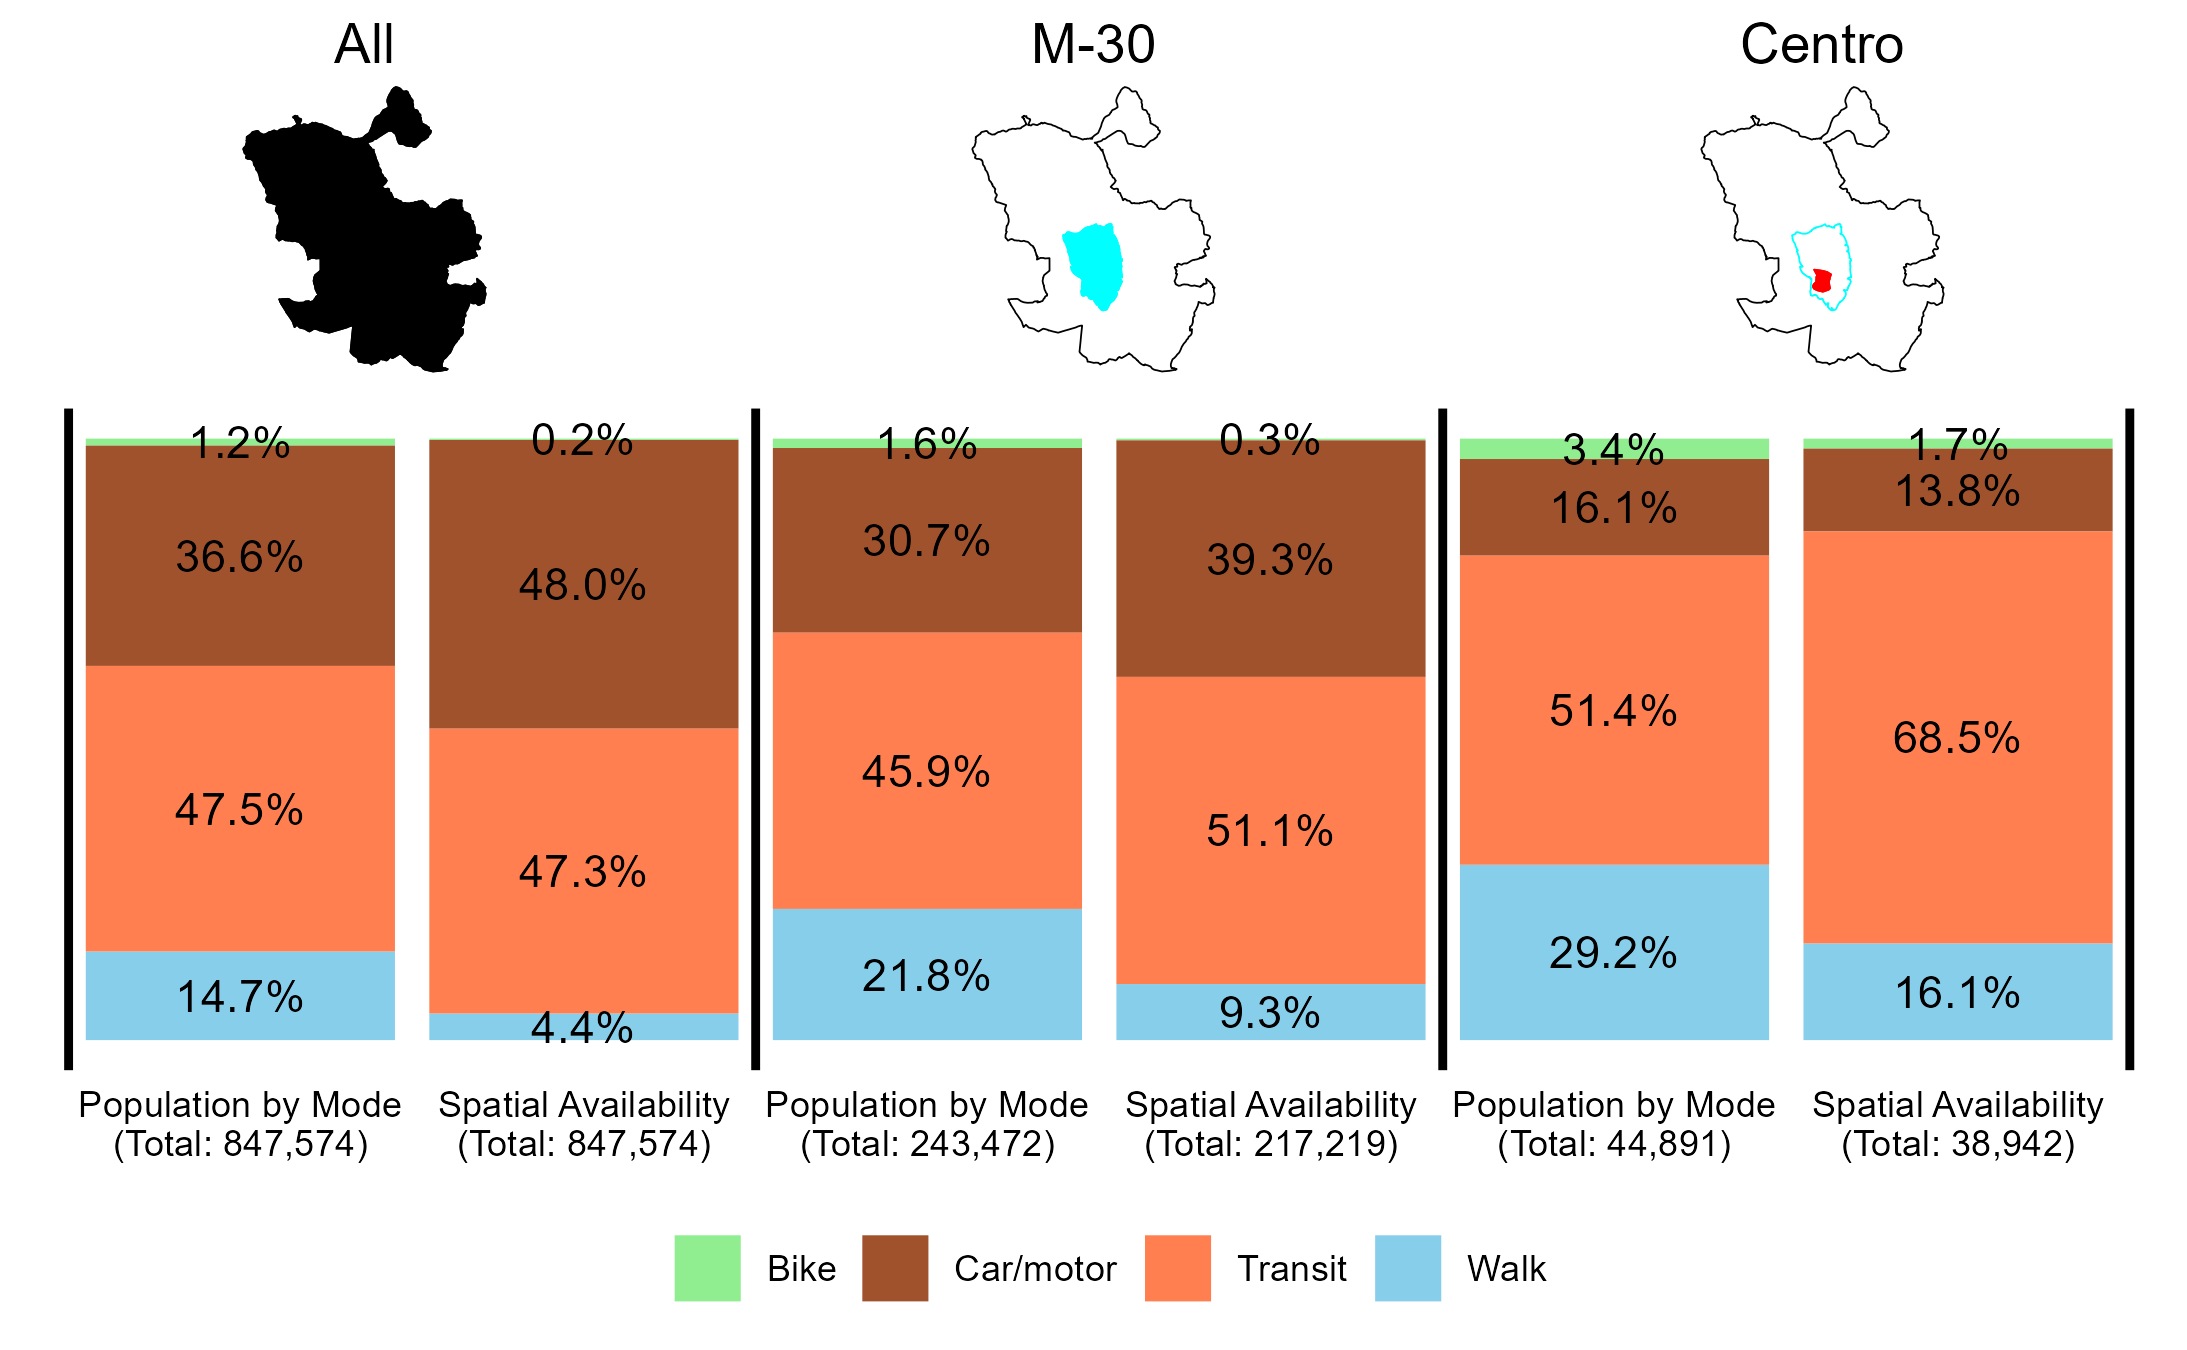
\includegraphics[width=1\linewidth]{images/modal_V_comps_4plot} 

}

\caption{\label{fig:Fig6} Displays the proportion of the working population by mode and spatial availability of job opportunities by mode aggregated for three spatial areas. From left to right, the city of Madrid (All), the area within the M-30 highway (M-30),the area within the Centro region (Centro).}\label{fig:modal-V-comps-plot}
\end{figure}

There are spatial variations in the competitive advantage of the
car-using populations. The proportion of car-using population in the
Centro is smaller and has higher travel impedance values relative to the
inputs in other areas and mode-using populations. The LEZ Centro
implementation further restricts the car-advantage as it shifted more
than half of all car trips into the LEZ to another mode {[}37{]}. This
restriction decreased the number of car-using population from \(i\)s
going into the LEZ Centro (an area with a large number of jobs overall,
see Figure \ref{fig:Fig2}), thus increasing the mass effect for non-car
modes and resulting in proportionally higher \(v_i^m\) values for
non-car modes. As such, the lower amount of access to opportunities by
car-mode allows more opportunities in the LEZ to be available by
populations using other modes.

As summarized in the two right-most columns in Figure \ref{fig:Fig6},
the proportion of spatial availability allocated to the car-using
population in the Centro (13.8\% or 5,373 opportunities). As a
comparative reference, this is less than the proportion of the car-using
population in the Centro (16.1\%), evidently less then the proportion of
car-using population in the city, and is the opposite of the trend
overall (left-most columns) and within the M-30 (middle columns). More
opportunities are spatial availability to non-car using populations
within the Centro, particularly transit-using populations (68.5\% of
spatially available jobs in the Centro despite representing 51.4\% of
the population in the Centro and 47.5\% in the city overall).

From Figure \ref{fig:Fig6}, it is also summarized that there is a higher
proportion of opportunities spatially available to walking and cycling
populations in the Centro than in the City overall and in all areas
within the M-30. Notably, within the Centro, 1.7\% and 16.1\% of
opportunities are spatially available to bike and walk modes
respectively, while their populations represent smaller proportions of
1.2\% and 14.7\% of the population overall. Though the proportion of
spatial availability for these mode-using populations is still lower
than the proportion of mode-using population located in the Centro,
these modes are more competitive within the Centro than outside of the
Centro. By restricting the more competitive car mode through the LEZ,
the advantage in the spatial availability of opportunities afforded to
the otherwise lesser competitive modes is made apparent.

The spatial differences in the competitive dis/advantage of spatial
availability between modes can also be visualized per origin. Figure
\ref{fig:Fig7} visualizes \(v_i^m\), the spatial availability \(V_i^m\)
divided by the mode-population. \(v_i^m\) values above 1 are represented
in increasing red shades, values below 1 are represented in increasingly
green shades, and values equal to 1 are white. These plots illustrates
the discussion of the disproportionately high over-allocation of spatial
availability relative to the mode-using population in many of the
origins for the car/motor mode (bottom left plot, areas denoted with
green \(v_i^m\) values above 1). These plots also visualize areas that
disproportionately capture lower spatial availability (under 1),
represented in shades of red. It can be observed that the transit-using
population's spatial availability to jobs is relatively balanced (i.e.,
many zones are white), while the non-motorized modes \(v_i^m\) values
are low (under 1) overall.

\begin{figure}

{\centering 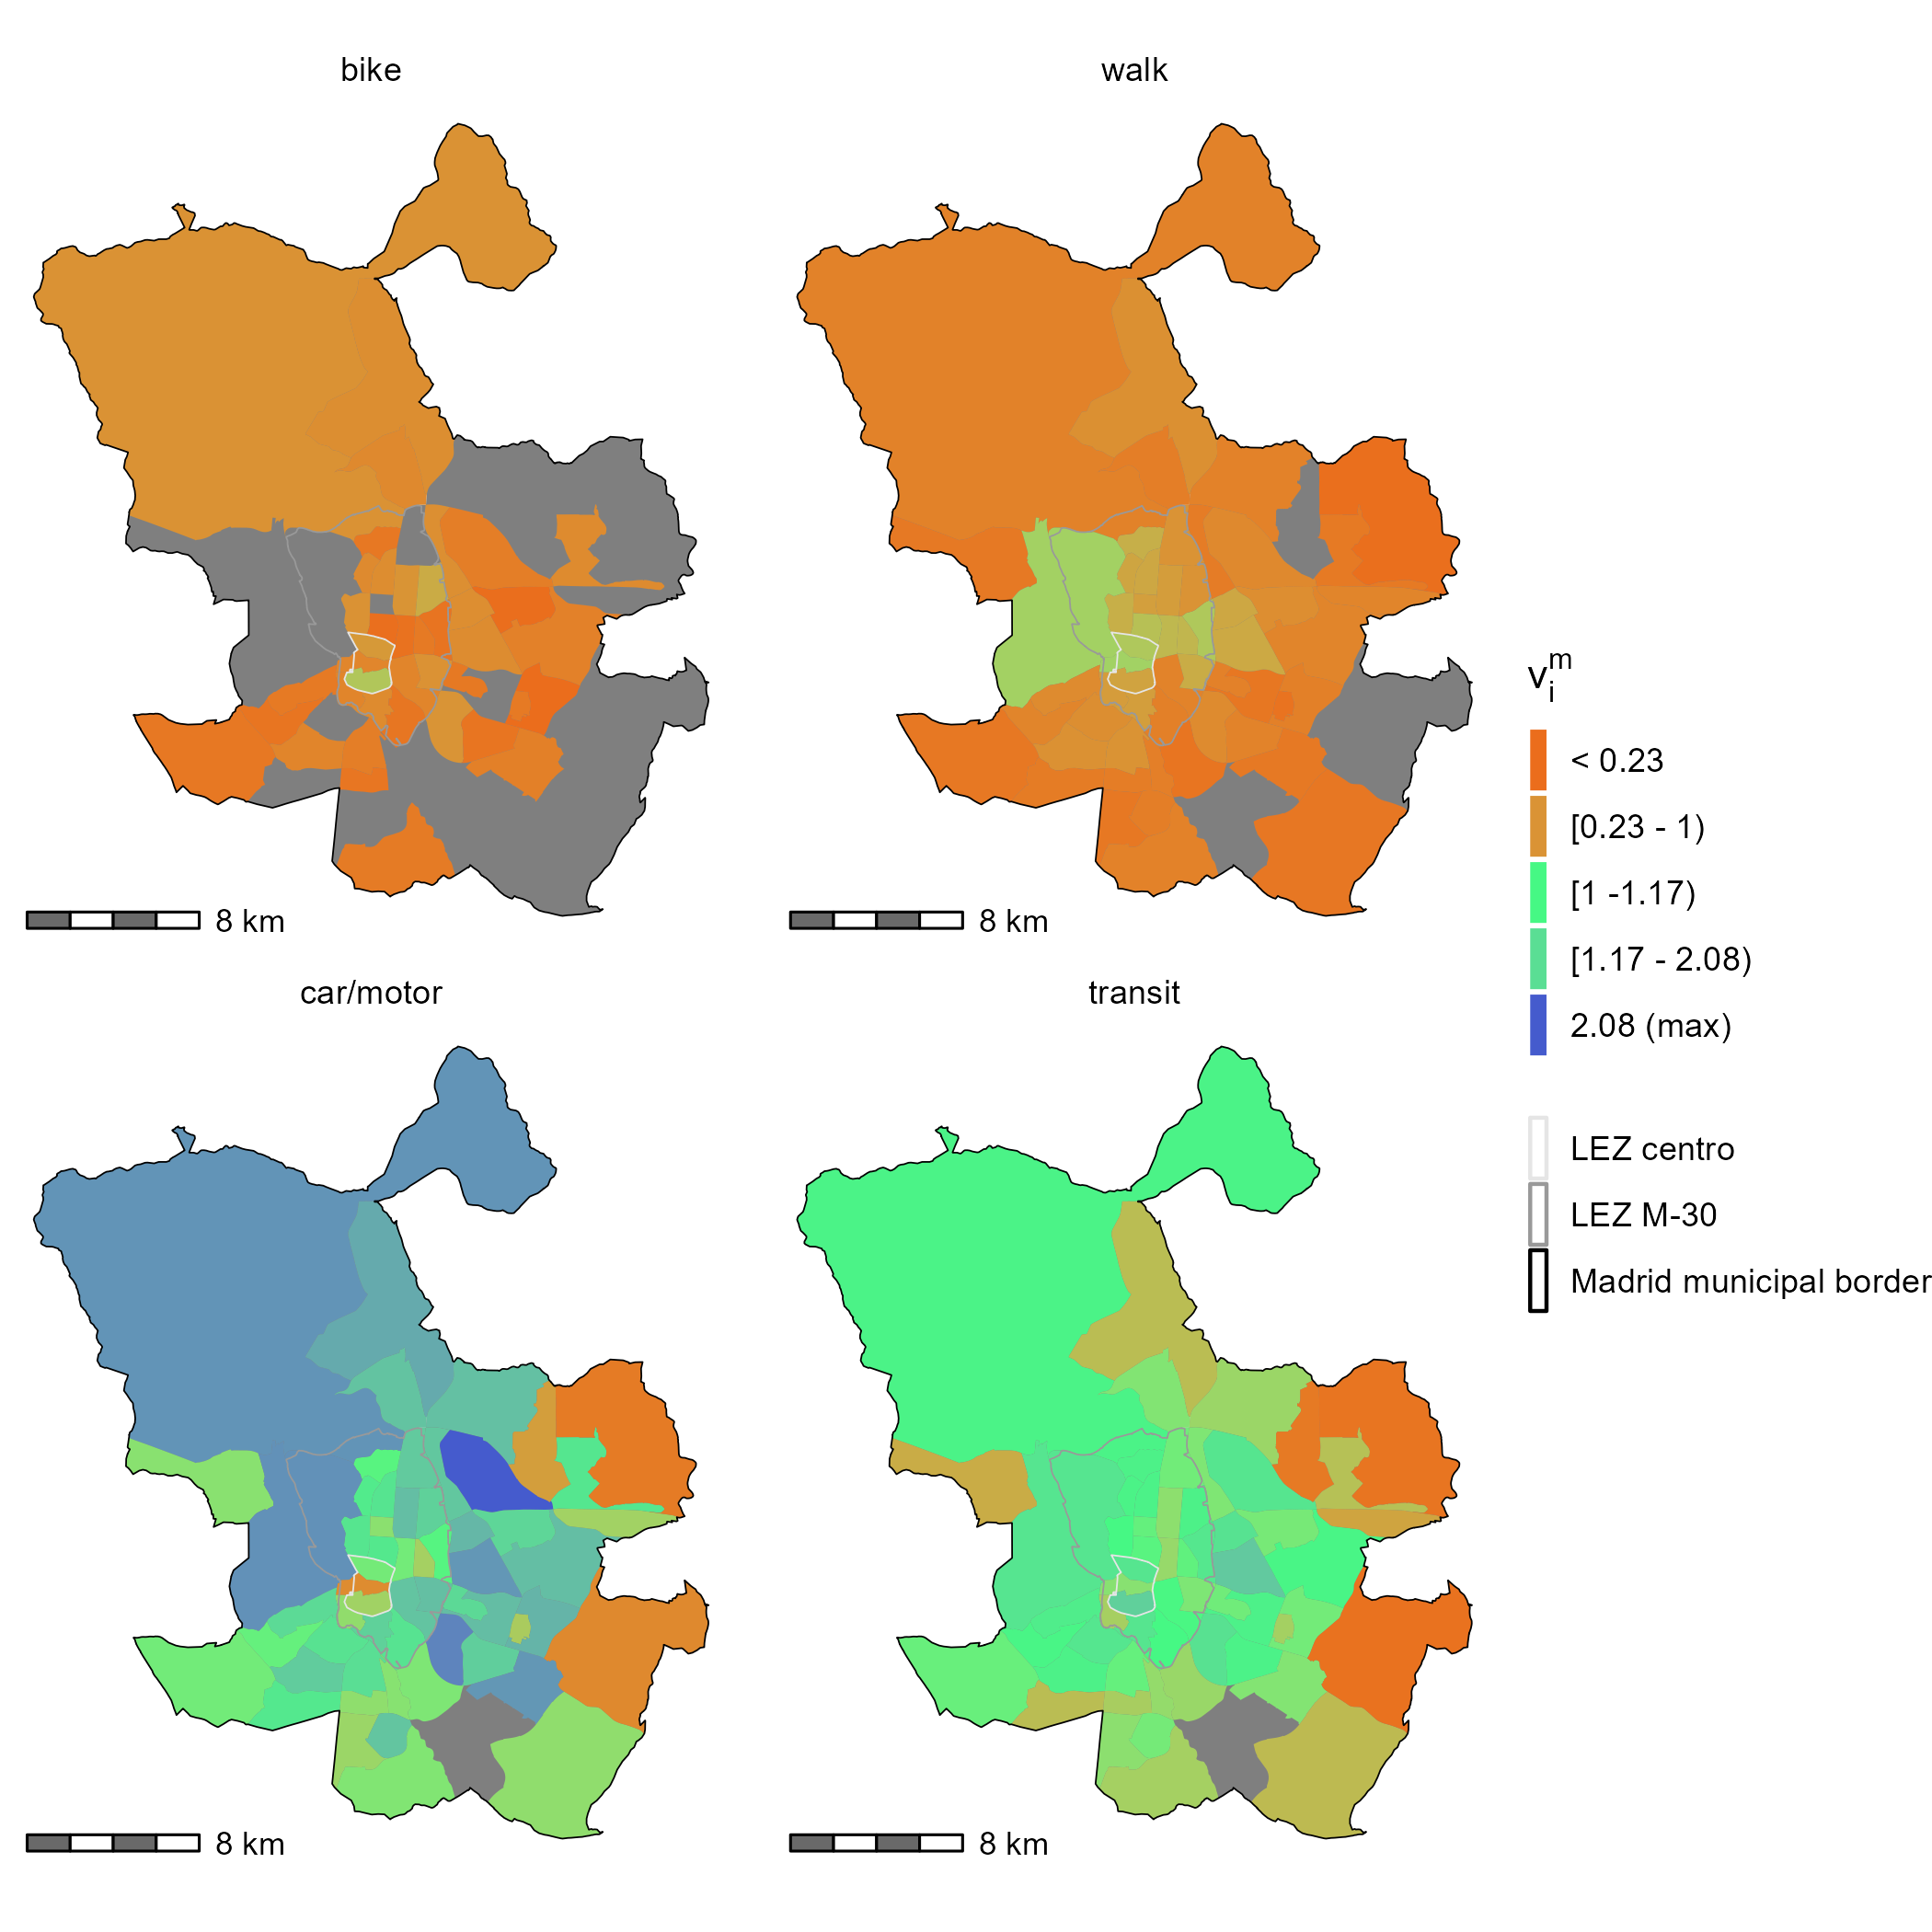
\includegraphics[width=1\linewidth]{images/SA_im_vv_zn208_plot} 

}

\caption{\label{fig:Fig7} Spatial availability of job opportunities per mode-using capita by mode $v_i^m$ per origin in Madrid. Calculated using the home-to-work flows from the 2018 travel survey. Gray TAZs have no population.}\label{fig:SA-per-capita-m-plot}
\end{figure}

Interestingly, as also represented in Figure \ref{fig:Fig6}, \(v_i^m\)
for car/motor within and near the LEZ Centro is near or below 1
(white/red) in Figure \ref{fig:Fig7} while all non-car modes have
relatively higher \(v_i^m\) values. Though the spatial availability from
before the LEZ Centro implementation is unknown, Figure \ref{fig:Fig7}
provides a benchmark for quantifying potential LEZ implementations in
the future (given 2018 travel conditions). Figure \ref{fig:Fig7} also
shows that many areas within the M-30 have high (white/green) \(v_i^m\)
values for car-mode, signaling that the spatial expansion of the LEZ
Centro stands to increase the spatial availability of jobs for non-car
mode using populations.

\hypertarget{discussion-and-conclusions}{%
\section{Discussion and conclusions}\label{discussion-and-conclusions}}

Location-based accessibility measures like the Hansen-type \(S_i^m\),
Shen-type \(a_i^m\), and spatial availability \(V_i^m\) measures share a
commonality; they are a weighted sum of opportunities assigned to each
spatial unit \(i\) in a region. In this way, they all can be interpreted
as a score of how many opportunities can be potentially interacted with
by the population at \(i\). How the weight and sum of the
potentially-interacted-with opportunities is considered is what defines
the type of accessibility measure.

Within this paper, the location-based singly- \emph{constrained} and
\emph{competitive} accessibility measure, known as spatial availability
\(V_i\) {[}14{]}, is extended for the case of capturing multimodal
accessibility to opportunities \(V_i^m\). A synthetic example and then
an empirical case of LEZ in Madrid are detailed to demonstrate this
multimodal extension.

The spatial availability measure is capable of capturing a new
interpretation of multimodal competition that previous accessibility
measures have not yet done. Competitive measures hypothesis that
populations using modes with lower travel impedance, when competing for
a finite set of opportunities, will capture more opportunities. With
spatial availability, the number of opportunities that are captured (of
the total opportunities in the region) by each mode can be individually
calculated. From there, the difference between how many spatially
available opportunities one mode captures versus another can be
investigated. This is the advantage of the spatial availability measure,
particularly its multimodal extension.

The flexibility and need for an accessibility measure such as spatial
availability is pertinent in policy scenario evaluation. As showcased in
the empirical example of the LEZ in Madrid, competition for job
opportunity availability varies spatially \emph{as well as} between
modes. The car and transit modes have the highest spatial availability,
with the car-mode having highest availability with exception to the
areas within the LEZ Centro. Since car travel has been highly restricted
within the LEZ Centro, fewer car-using people potentially interact with
jobs within the LEZ Centro, leaving more \emph{spatially available} jobs
for non-car-using populations. This difference in car-using populations
in locations accessing jobs within and immediately outside the LEZ
Centro increases the competitiveness of the transit-using population
(the second most competitive mode) as well as the non-motorized modes.

Spatial availability \(V_i^m\) can also be divided by the mode-using
population at each \(i\) to yield mode-population normalized values.
These values, reflected in Figure \ref{fig:Fig7}, can be used as a
benchmark to investigate existing conditions and plan future LEZ
implementation (i.e., target areas with exceptionally high car spatial
availability such that more opportunities are available to other
mode-users).

In summary, conventional \emph{non-constrained} accessibility measures
are difficult for planners to operationalize for a variety of reasons
including issues of computation and interpretability {[}5{]}. With
spatial availability, the magnitude of opportunities that are available
as a proportion of all the opportunities in the region is equal to
\(V_i\). As a result of its proportional allocation mechanism, \(V_i\)
can be naturally extended into multimodal applications. This flexibility
is helpful to modelling policy scenarios in our cities that are
increasingly multimodal. The interpretation of \(V_i\) allows for
manipulation of \(V_i^m\) values to investigate differences of
availability between neighbourhoods, modes, and regions, generate per
capita benchmarks, and/or generate average values per population-group.

From a spatial equity perspective, spatial availability measure can
provide researchers, policy makers, and citizens a new-found
interpretation of accessibility measures. With a plot of spatial
availability values, one can begin asking, how much is enough and what
level may be too much. These interpretations were difficult to be made
with accessibility measures in the past. In future work, we intend to
use multimodal spatial availability to characterise the equity of
multimodal accessibility losses and gains in varying LEZ policy scenario
implementations.

\hypertarget{acknowledgements}{%
\section{Acknowledgements}\label{acknowledgements}}

This research was funded by the Canada Graduate Scholarship - Doctoral
Program (CGS D) provided by the Social Sciences and Humanities Research
Council (SSHRC) and Project Mobilizing Justice, also supported by SSHRC.
The funders had no role in study design, data collection and analysis,
decision to publish, or preparation of the manuscript.

All work is fully-reproducible and available within this
\href{https://github.com/soukhova/Multimodal-spatial-availability}{GitHub
repository}.

\hypertarget{author-contributions}{%
\section{Author contributions}\label{author-contributions}}

The authors confirm contribution to the paper as follows: study
conception and design: AS, JTO, JSL, AP.; data collection: AS, JTO,
JSL.; analysis and interpretation of results: AS, JTO, JSL, AP.; draft
manuscript preparation: AS, JSL, AP. All authors reviewed the results
and approved the final version of the manuscript.

\hypertarget{references}{%
\section*{References}\label{references}}
\addcontentsline{toc}{section}{References}

\hypertarget{refs}{}
\begin{CSLReferences}{0}{0}
\leavevmode\vadjust pre{\hypertarget{ref-hansenHowAccessibilityShapes1959}{}}%
\CSLLeftMargin{1. }%
\CSLRightInline{Hansen WG. How accessibility shapes land use. Journal of
the American Institute of Planners. 1959;25: 73--76.
doi:\href{https://doi.org/10.1080/01944365908978307}{10.1080/01944365908978307}}

\leavevmode\vadjust pre{\hypertarget{ref-geursAccessibility2004}{}}%
\CSLLeftMargin{2. }%
\CSLRightInline{Geurs KT, Wee B van. Accessibility evaluation of
land-use and transport strategies: Review and research directions.
Journal of Transport Geography. 2004;12: 127--140. Available:
\href{http://www.sciencedirect.com/science/article/B6VG8-4B28VY7-1/2/61478339c14cab4fa58438ad7b1f4610\%0AC:/Papers/Journal\%20of\%20Transport\%20Geography/Journal\%20of\%20Transport\%20Geography\%20(2004)\%2012\%20(2)\%20127-140.pdf}{http://www.sciencedirect.com/science/article/B6VG8-4B28VY7-1/2/61478339c14cab4fa58438ad7b1f4610
C:/Papers/Journal of Transport Geography/Journal of Transport Geography
(2004) 12 (2) 127-140.pdf}}

\leavevmode\vadjust pre{\hypertarget{ref-paezPositive2012}{}}%
\CSLLeftMargin{3. }%
\CSLRightInline{Paez A, Scott DM, Morency C. Measuring accessibility:
Positive and normative implementations of various accessibility
indicators. Journal of Transport Geography. 2012;25: 141--153.
doi:\href{https://doi.org/10.1016/j.jtrangeo.2012.03.016}{10.1016/j.jtrangeo.2012.03.016}}

\leavevmode\vadjust pre{\hypertarget{ref-handyAccessibility2020}{}}%
\CSLLeftMargin{4. }%
\CSLRightInline{Handy S. Is accessibility an idea whose time has finally
come? Transportation Research Part D: Transport and Environment.
2020;83: 102319. doi:\url{https://doi.org/10.1016/j.trd.2020.102319}}

\leavevmode\vadjust pre{\hypertarget{ref-levinsonTransportAccessManual2020}{}}%
\CSLLeftMargin{5. }%
\CSLRightInline{Levinson D, King D. Transport access manual: {A} guide
for measuring connection between people and places. {University of
Sydney}; 2020. Available:
\url{https://ses.library.usyd.edu.au/handle/2123/23733}}

\leavevmode\vadjust pre{\hypertarget{ref-siddiqToolsTradeAssessing2021}{}}%
\CSLLeftMargin{6. }%
\CSLRightInline{Siddiq F, D. Taylor B. Tools of the trade?: Assessing
the progress of accessibility measures for planning practice. Journal of
the American Planning Association. 2021;87: 497--511.
doi:\href{https://doi.org/10.1080/01944363.2021.1899036}{10.1080/01944363.2021.1899036}}

\leavevmode\vadjust pre{\hypertarget{ref-yanAccessibilityBasedPlanningAddressing2021}{}}%
\CSLLeftMargin{7. }%
\CSLRightInline{Yan X. Toward accessibility-based planning addressing
the myth of travel cost savings. {JOURNAL} {OF} {THE} {AMERICAN}
{PLANNING} {ASSOCIATION}. 2021;87: 409--423.
doi:\href{https://doi.org/10.1080/01944363.2020.1850321}{10.1080/01944363.2020.1850321}}

\leavevmode\vadjust pre{\hypertarget{ref-elGeneidyMaking2022}{}}%
\CSLLeftMargin{8. }%
\CSLRightInline{El-Geneidy A, Levinson D. Making accessibility work in
practice. Transport Reviews. 2022;42: 129--133.
doi:\href{https://doi.org/10.1080/01441647.2021.1975954}{10.1080/01441647.2021.1975954}}

\leavevmode\vadjust pre{\hypertarget{ref-handyMeasuring1997}{}}%
\CSLLeftMargin{9. }%
\CSLRightInline{Handy S, Niemeier D. Measuring accessibility: An
exploration of issues and alternatives. Environment and Planning A.
1997;29: 1175--1194. }

\leavevmode\vadjust pre{\hypertarget{ref-kwanSpace1998}{}}%
\CSLLeftMargin{10. }%
\CSLRightInline{Kwan MP. Space-time and integral measures of individual
accessibility: A comparative analysis using a point-based framework.
Geographical Analysis. 1998;30: 191--216. Available:
\href{https://ISI:000074579200001\%0AC:/Papers/Geographical\%20Analysis/Geographical\%20Analysis\%20(1998)\%2030\%20(3)\%20191-216.pdf}{ISI:000074579200001
C:/Papers/Geographical Analysis/Geographical Analysis (1998) 30 (3)
191-216.pdf}}

\leavevmode\vadjust pre{\hypertarget{ref-shenLocationCharacteristicsInnercity1998}{}}%
\CSLLeftMargin{11. }%
\CSLRightInline{Shen Q. Location characteristics of inner-city
neighborhoods and employment accessibility of low-wage workers. Environ
Plann B. 1998;25: 345--365.
doi:\href{https://doi.org/10.1068/b250345}{10.1068/b250345}}

\leavevmode\vadjust pre{\hypertarget{ref-luoMeasuresSpatialAccessibility2003}{}}%
\CSLLeftMargin{12. }%
\CSLRightInline{Luo W, Wang F. Measures of spatial accessibility to
health care in a {GIS} environment: Synthesis and a case study in the
chicago region. Environ Plann B Plann Des. 2003;30: 865--884.
doi:\href{https://doi.org/10.1068/b29120}{10.1068/b29120}}

\leavevmode\vadjust pre{\hypertarget{ref-paezDemand2019}{}}%
\CSLLeftMargin{13. }%
\CSLRightInline{Paez A, Higgins CD, Vivona SF. Demand and level of
service inflation in floating catchment area (FCA) methods. PloS one.
2019;14: e0218773.
doi:\href{https://doi.org/10.1371/journal.pone.0218773}{10.1371/journal.pone.0218773}}

\leavevmode\vadjust pre{\hypertarget{ref-soukhovIntroducingSpatialAvailability2023}{}}%
\CSLLeftMargin{14. }%
\CSLRightInline{Soukhov A, Paez A, Higgins CD, Mohamed M. Introducing
spatial availability, a singly-constrained measure of competitive
accessibility {\textbar} {PLOS} {ONE}. {PLOS} {ONE}. 2023; 1--30.
doi:\href{https://\%20doi.org/10.1371/journal.pone.0278468}{https://
doi.org/10.1371/journal.pone.0278468}}

\leavevmode\vadjust pre{\hypertarget{ref-paezHealth2010}{}}%
\CSLLeftMargin{15. }%
\CSLRightInline{Páez A, Mercado R, Farber S, Morency C, Roorda M.
Accessibility to health care facilities in montreal island: An
application of relative accessibility indicators from the perspective of
senior and non-senior residents. International Journal of Health
Geographics. 2010;9: 1--9. Available:
\url{http://www.ij-healthgeographics.com/content/9/1/52}}

\leavevmode\vadjust pre{\hypertarget{ref-moniruzzamanMode2013}{}}%
\CSLLeftMargin{16. }%
\CSLRightInline{Moniruzzaman M, Páez A, Nurul Habib KM, Morency C. Mode
use and trip length of seniors in montreal. Journal of Transport
Geography. 2013;30: 89--99.
doi:\url{http://dx.doi.org/10.1016/j.jtrangeo.2013.03.007}}

\leavevmode\vadjust pre{\hypertarget{ref-reyesWalking2014}{}}%
\CSLLeftMargin{17. }%
\CSLRightInline{Reyes M, Paez A, Morency C. Walking accessibility to
urban parks by children: A case study of montreal. Landscape and Urban
Planning. 2014;125: 38--47.
doi:\href{https://doi.org/10.1016/j.landurbplan.2014.02.002}{10.1016/j.landurbplan.2014.02.002}}

\leavevmode\vadjust pre{\hypertarget{ref-paezJobs2013}{}}%
\CSLLeftMargin{18. }%
\CSLRightInline{Páez A, Farber S, Mercado R, Roorda M, Morency C. Jobs
and the single parent: An analysis of accessibility to employment in
toronto. Urban Geography. 2013;34: 815--842.
doi:\href{https://doi.org/10.1080/02723638.2013.778600}{10.1080/02723638.2013.778600}}

\leavevmode\vadjust pre{\hypertarget{ref-wuUnifyingAccess2020}{}}%
\CSLLeftMargin{19. }%
\CSLRightInline{Wu H, Levinson D. Unifying access. Transportation
Research Part D: Transport and Environment. 2020;83: 102355.
doi:\href{https://doi.org/10.1016/j.trd.2020.102355}{10.1016/j.trd.2020.102355}}

\leavevmode\vadjust pre{\hypertarget{ref-tahmasbiMultimodalAccessibilitybasedEquity2019}{}}%
\CSLLeftMargin{20. }%
\CSLRightInline{Tahmasbi B, Mansourianfar MH, Haghshenas H, Kim I.
Multimodal accessibility-based equity assessment of urban public
facilities distribution. Sustainable Cities and Society. 2019;49:
101633.
doi:\href{https://doi.org/10.1016/j.scs.2019.101633}{10.1016/j.scs.2019.101633}}

\leavevmode\vadjust pre{\hypertarget{ref-campbell2019accessibility}{}}%
\CSLLeftMargin{21. }%
\CSLRightInline{Campbell KB, Rising JA, Klopp JM, Mbilo JM.
Accessibility across transport modes and residential developments in
nairobi. Journal of Transport Geography. 2019;74: 77--90. }

\leavevmode\vadjust pre{\hypertarget{ref-maharjanSpatialEquityModal2022}{}}%
\CSLLeftMargin{22. }%
\CSLRightInline{Maharjan S, Tilahun N, Ermagun A. Spatial equity of
modal access gap to multiple destination types across chicago. Journal
of Transport Geography. 2022;104: 103437.
doi:\href{https://doi.org/10.1016/j.jtrangeo.2022.103437}{10.1016/j.jtrangeo.2022.103437}}

\leavevmode\vadjust pre{\hypertarget{ref-lunkeModalAccessibilityDisparities2022}{}}%
\CSLLeftMargin{23. }%
\CSLRightInline{Lunke EB. Modal accessibility disparities and transport
poverty in the oslo region. Transportation Research Part D: Transport
and Environment. 2022;103: 103171.
doi:\href{https://doi.org/10.1016/j.trd.2022.103171}{10.1016/j.trd.2022.103171}}

\leavevmode\vadjust pre{\hypertarget{ref-grengsJobAccessibilityModal2010}{}}%
\CSLLeftMargin{24. }%
\CSLRightInline{Grengs J. Job accessibility and the modal mismatch in
detroit. Journal of Transport Geography. 2010;18: 42--54.
doi:\href{https://doi.org/10.1016/j.jtrangeo.2009.01.012}{10.1016/j.jtrangeo.2009.01.012}}

\leavevmode\vadjust pre{\hypertarget{ref-kawabataJobAccessibilityIndicator2006}{}}%
\CSLLeftMargin{25. }%
\CSLRightInline{Kawabata M, Shen Q. Job accessibility as an indicator of
auto-oriented urban structure: A comparison of boston and los angeles
with tokyo. Environ Plann B Plann Des. 2006;33: 115--130.
doi:\href{https://doi.org/10.1068/b31144}{10.1068/b31144}}

\leavevmode\vadjust pre{\hypertarget{ref-kwokUseModalAccessibility2004}{}}%
\CSLLeftMargin{26. }%
\CSLRightInline{Kwok RCW, Yeh AGO. The use of modal accessibility gap as
an indicator for sustainable transport development. Environ Plan A.
2004;36: 921--936.
doi:\href{https://doi.org/10.1068/a3673}{10.1068/a3673}}

\leavevmode\vadjust pre{\hypertarget{ref-morrisAccessibilityIndicatorsTransport1979}{}}%
\CSLLeftMargin{27. }%
\CSLRightInline{Morris JM, Dumble PL, Wigan MR. Accessibility indicators
for transport planning. Transportation Research Part A: General.
1979;13: 91--109.
doi:\href{https://doi.org/10.1016/0191-2607(79)90012-8}{10.1016/0191-2607(79)90012-8}}

\leavevmode\vadjust pre{\hypertarget{ref-weibullAxiomaticApproachMeasurement1976}{}}%
\CSLLeftMargin{28. }%
\CSLRightInline{Weibull JW. An axiomatic approach to the measurement of
accessibility. Regional Science and Urban Economics. 1976;6: 357--379.
doi:\href{https://doi.org/10.1016/0166-0462(76)90031-4}{10.1016/0166-0462(76)90031-4}}

\leavevmode\vadjust pre{\hypertarget{ref-josephMeasuringPotentialPhysical1982}{}}%
\CSLLeftMargin{29. }%
\CSLRightInline{Joseph AE, Bantock PR. Measuring potential physical
accessibility to general practitioners in rural areas: A method and case
study. Social Science \& Medicine. 1982;16: 85--90.
doi:\href{https://doi.org/10.1016/0277-9536(82)90428-2}{10.1016/0277-9536(82)90428-2}}

\leavevmode\vadjust pre{\hypertarget{ref-taoInvestigatingImpactsPublic2020a}{}}%
\CSLLeftMargin{30. }%
\CSLRightInline{Tao Z, Zhou J, Lin X, Chao H, Li G. Investigating the
impacts of public transport on job accessibility in {Shenzhen}, {China}:
A multi-modal approach. Land Use Policy. 2020;99: 105025.
doi:\href{https://doi.org/10.1016/j.landusepol.2020.105025}{10.1016/j.landusepol.2020.105025}}

\leavevmode\vadjust pre{\hypertarget{ref-carpentieriMultimodalAccessibilityPrimary2020}{}}%
\CSLLeftMargin{31. }%
\CSLRightInline{Carpentieri G, Guida C, Masoumi HE. Multimodal
{Accessibility} to {Primary Health Services} for the {Elderly}: {A Case
Study} of {Naples}, {Italy}. Sustainability. 2020;12: 781.
doi:\href{https://doi.org/10.3390/su12030781}{10.3390/su12030781}}

\leavevmode\vadjust pre{\hypertarget{ref-margaryanLowEmissionZones2021}{}}%
\CSLLeftMargin{32. }%
\CSLRightInline{Margaryan S. Low emission zones and population health.
Journal of Health Economics. 2021;76: 102402.
doi:\href{https://doi.org/10.1016/j.jhealeco.2020.102402}{10.1016/j.jhealeco.2020.102402}}

\leavevmode\vadjust pre{\hypertarget{ref-verbeekJustManagementUrban2022}{}}%
\CSLLeftMargin{33. }%
\CSLRightInline{Verbeek T, Hincks S. The {``just''} management of urban
air pollution? A geospatial analysis of low emission zones in brussels
and london. Applied Geography. 2022;140: 102642.
doi:\href{https://doi.org/10.1016/j.apgeog.2022.102642}{10.1016/j.apgeog.2022.102642}}

\leavevmode\vadjust pre{\hypertarget{ref-espanaPlanNacionalIntegrado2020}{}}%
\CSLLeftMargin{34. }%
\CSLRightInline{España. Plan nacional integrado de energía y clima
({PNIEC}) 2021-2030. 2020 {[}cited 30 Jul 2023{]}. Available:
\url{https://www.miteco.gob.es/es/prensa/pniec.html}}

\leavevmode\vadjust pre{\hypertarget{ref-espanaResolucion10Enero2020}{}}%
\CSLLeftMargin{35. }%
\CSLRightInline{España. Resolución de 10 de enero de 2020, de la
dirección general de biodiversidad y calidad ambiental, por la que se
publica el programa nacional de control de la contaminación atmosférica.
Resolución Jan 24, 2020 pp. 6947--6947. Available:
\url{https://www.boe.es/eli/es/res/2020/01/10/(10)}}

\leavevmode\vadjust pre{\hypertarget{ref-barcelonaGUIATECNICAPARA2021}{}}%
\CSLLeftMargin{36. }%
\CSLRightInline{Barcelona. {GUÍA} {TÉCNICA} {PARA} {LA} {IMPLEMENTACIÓN}
{DE} {ZONAS} {DE} {BAJAS} {EMISIONES}. Àrea Metropolitana de Barcelona
({AMB}): Oficina Técnica de Gerencia del {AMB}; 2021. Available:
\url{https://revista.dgt.es/images/GUIA-ZBE.pdf}}

\leavevmode\vadjust pre{\hypertarget{ref-tarrinoortizAnalyzingImpactLow2022}{}}%
\CSLLeftMargin{37. }%
\CSLRightInline{Tarriño-Ortiz J, Gómez J, Soria-Lara JA, Vassallo JM.
Analyzing the impact of low emission zones on modal shift. Sustainable
Cities and Society. 2022;77: 103562.
doi:\href{https://doi.org/10.1016/j.scs.2021.103562}{10.1016/j.scs.2021.103562}}

\leavevmode\vadjust pre{\hypertarget{ref-comunidaddemadridResultadosEDM20182020}{}}%
\CSLLeftMargin{38. }%
\CSLRightInline{Comunidad de Madrid. Resultados de la {EDM} 2018 - Datos
Abiertos. 2020 {[}cited 31 Jul 2023{]}. Available:
\url{https://datos.comunidad.madrid/catalogo/dataset/resultados-edm2018}}

\leavevmode\vadjust pre{\hypertarget{ref-lopez_2017_spatial}{}}%
\CSLLeftMargin{39. }%
\CSLRightInline{Lopez FA, Paez A. Spatial clustering of high-tech
manufacturing and knowledge-intensive service firms in the greater
toronto area. Canadian Geographer-Geographe Canadien. 2017;61: 240--252.
doi:\href{https://doi.org/10.1111/cag.12326}{10.1111/cag.12326}}

\leavevmode\vadjust pre{\hypertarget{ref-horbachov_theoretical_2018}{}}%
\CSLLeftMargin{40. }%
\CSLRightInline{Horbachov P, Svichynskyi S. Theoretical substantiation
of trip length distribution for home-based work trips in urban transit
systems. Journal of Transport and Land Use. 2018;11: 593--632.
Available: \url{https://www.jstor.org/stable/26622420}}

\leavevmode\vadjust pre{\hypertarget{ref-batista_estimation_2019}{}}%
\CSLLeftMargin{41. }%
\CSLRightInline{Batista SFA, Leclercq L, Geroliminis N. Estimation of
regional trip length distributions for the calibration of the aggregated
network traffic models. Transportation Research Part B: Methodological.
2019;122: 192--217.
doi:\href{https://doi.org/10.1016/j.trb.2019.02.009}{10.1016/j.trb.2019.02.009}}

\leavevmode\vadjust pre{\hypertarget{ref-fitdistrplus_2015}{}}%
\CSLLeftMargin{42. }%
\CSLRightInline{Delignette-Muller ML, Dutang C. {fitdistrplus}: An {R}
package for fitting distributions. Journal of Statistical Software.
2015;64: 1--34. Available:
\url{https://www.jstatsoft.org/article/view/v064i04}}

\leavevmode\vadjust pre{\hypertarget{ref-reggianiAccessibilityImpedanceForms2011}{}}%
\CSLLeftMargin{43. }%
\CSLRightInline{Reggiani A, Bucci P, Russo G. Accessibility and
impedance forms: Empirical applications to the german commuting network.
International Regional Science Review. 2011;34: 230--252.
doi:\href{https://doi.org/10.1177/0160017610387296}{10.1177/0160017610387296}}

\leavevmode\vadjust pre{\hypertarget{ref-soukhovTTS2016RDataSet2023}{}}%
\CSLLeftMargin{44. }%
\CSLRightInline{Soukhov A, Páez A. {TTS}2016R: A data set to study
population and employment patterns from the 2016 transportation tomorrow
survey in the greater golden horseshoe area, ontario, canada.
Environment and Planning B: Urban Analytics and City Science. 2023;
23998083221146781.
doi:\href{https://doi.org/10.1177/23998083221146781}{10.1177/23998083221146781}}

\end{CSLReferences}

\nolinenumbers



\end{document}
